\documentclass[a4paper,12pt]{report}

% Pacotes necessários
\usepackage[utf8]{inputenc}
\usepackage[brazil]{babel}
\usepackage{hyperref}
\usepackage[T1]{fontenc}
\usepackage{graphicx}
\usepackage{caption}
\usepackage[left=2cm, right=2cm, top=2cm, bottom=2cm]{geometry}
\usepackage{lipsum} % Para gerar texto de preenchimento
\usepackage{float}
\usepackage{amsmath}
\usepackage{listings}


% Configuração da página de título
\newcommand{\reporttitle}{Trabalho 1 - Reator}
\newcommand{\reportauthor}{
Lucas William Junges}
\newcommand{\reportdate}{30/06/2025}
%\renewcommand{\listoffigures}{}
%\renewcommand{\tableofcontents}{}

\begin{document}

% Página de título personalizada
\begin{titlepage}
    \centering
    \vspace*{1cm}
    
\includegraphics[width=0.4\textwidth]{Imagens/BrasaoUFSC.png} % Adicione o caminho para o logotipo da sua instituição
    \par\vspace{1cm}
    {\scshape\Large Universidade Federal de Santa Catarina\par} % Substitua pelo nome da sua instituição
    \vspace{1.2cm}
    {\huge\bfseries \reporttitle\par}
    \vspace{2cm}
    {\Large\itshape \reportauthor\par}
    \vfill
    {\large \reportdate\par}
\end{titlepage}

% Lista de ilustrações
\listoffigures
\clearpage

% Sumário
\tableofcontents
\clearpage

% Introdução
\chapter{Introdução}
\label{chap:introducao}

A presente pesquisa aborda o projeto e a análise de um sistema de controle de concentração de produto em um reator continuamente agitado, utilizado na indústria química para a produção de cyclopentenol (produto B) a partir de cyclopentadiene (produto A), com a presença de um catalisador diluído em água. Além do produto desejado, há a formação de dois produtos residuais, dicyclopentadiene (produto D) e cyclopentanediol (produto C).

A dinâmica do processo é regida por uma série de parâmetros, onde \( k_1 \), \( k_2 \) e \( k_3 \) são considerados constantes quando o reator opera à temperatura constante. A concentração desejada a ser controlada, \( C_b \), depende das concentrações de A no reator (\( C_a \)) e no fluido de alimentação (\( C_{af} \)), bem como da vazão de diluição (\( F \)). O sistema utiliza a variável manipulada \( u = F/V \), onde \( V \) é o volume do reator.

A pesquisa está estruturada em diversas partes. Inicialmente, será realizada uma análise do sistema em equilíbrio, com o desenho das características estáticas dentro das faixas de variação das variáveis envolvidas. Em seguida, utilizando Simulink, será estudado o comportamento dinâmico do sistema por simulação, verificando os pontos de equilíbrio encontrados no modelo estático. Será feito o estudo de linearização do sistema, a obtenção de modelos incrementais dinâmicos e a determinação de funções de transferência relacionando as variáveis manipulada e perturbação com as concentrações.

Posteriormente, será projetado um controle proporcional-integral (PI) contínuo utilizando a técnica de alocação de polos, buscando atender a especificações de tempo de estabilização e pico de resposta. Será feita uma análise das respostas em malha fechada do sistema para degraus de referência e perturbações, interpretando os resultados através de diagramas polo-zero e de resposta em frequência.

Continuará o estudo, simulando o comportamento dinâmico do sistema em malha fechada com o modelo completo não linear, avaliando se as especificações são atendidas. Será realizada uma análise da resposta ao sistema frente a variações próximas ao ponto de operação e perturbações.

Por fim, será discretizado o controle, implementando-o em MATLAB, e será analisado seu desempenho em comparação com o controle contínuo, observando o efeito da amostragem.

O objetivo principal desta pesquisa é compreender os princípios de controle e análise de sistemas dinâmicos aplicados a processos químicos industriais, utilizando ferramentas teóricas e de simulação para projetar e avaliar estratégias de controle eficazes.


% Desenvolvimento
\chapter{Desenvolvimento}
\label{chap:desenvolvimento}

A figura mostra um sistema de controle de concentração de produto em um reator continuamente agitado, 
usado na indústria química.


 \begin{figure}[ht]
  \centering
  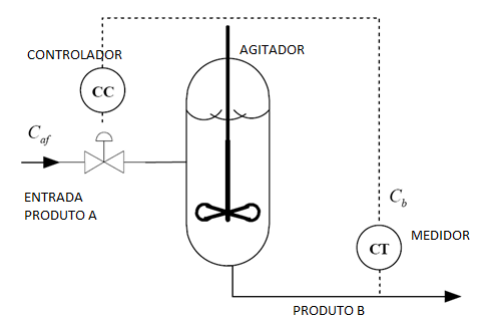
\includegraphics[width=0.6\textwidth]{Imagens/Reator.png}
 % \caption{Reator}
  \end{figure}

  Neste caso se produz cyclopentenol (produto B) a partir de cyclopentadiene (produto A) pela adição de um 
catalizador diluído em água. O sistema ainda produz dois produtos residuais dicyclopentadiene (produto D) 
e cyclopentanediol (produto C). A reação vem dada por:
  
\[ A \xrightarrow{k_1} B \xrightarrow{k_2} C \]
\[ 2A \xrightarrow{k_3} D\]

\[
\frac{dC_a(t)}{dt} = -k_1 C_a(t) - k_3 C_a(t)^2 + \frac{(C_{af}(t) - C_a(t)) F(t)}{V}
\]

\[
\frac{dC_b(t)}{dt} = k_1 C_a(t) - k_2 C_b(t) - \frac{C_b(t) F(t)}{V}
\]

Os parâmetros \( k_1 \), \( k_2 \) e \( k_3 \) são considerados constantes quando o reator trabalha à temperatura constante 
(\( k_1 = 6.01 \, \text{min}^{-1} \), \( k_2 = 0.8433 \, \text{min}^{-1} \), \( k_3 = 0.1123 \, \text{mol/(l min)} \)). 
A concentração que se quer controlar \( C_b \) (do produto \( B \)), depende de \( C_a \) e \( C_{af} \), que são as 
concentrações de \( A \) no reator e no fluido de alimentação, respectivamente, e também da vazão \( F \) 
(\( \text{l/min} \)) da diluição. \( V \) é o volume (\( \text{l} \)) do reator, que é constante.

O sistema usa \( u = F/V \) como variável manipulada e \( C_{af} \), a concentração da entrada, é a principal perturbação. 
\( u \) pode variar entre \( 0 \) e \( 10 \, \text{l/min} \), e a concentração de entrada \( C_{af} \) entre \( 4.0 \) e \( 6 \, \text{mol/L} \).



\section*{Parte 1 -  Análise do Sistema e Projeto por Alocação}
\section{1) Análise do Funcionamento do Sistema em Equilíbrio}

Analise o funcionamento do sistema em equilíbrio desenhando as características estáticas dentro da faixa de variação das diferentes variáveis envolvidas.

Isolando os termos em comum:

\begin{align}
\frac{dC_a}{dt} &= -k_1 C_a(t) - k_3 C_a(t)^2 + \frac{(C_{a_f}(t)- C_a(t))F(t)}{V} \\
\frac{dC_a}{dt} &= C_a(-k_1 - k_3 C_a -  \frac{F(t)}{V})+\frac{C_{a_f} F(t)}{V} \\
\\
\frac{dC_b}{dt} &= k_1 C_a - k_2 C_b - \frac{C_b F}{V} \\
\frac{dC_b}{dt} &= k_1 C_a + C_b(-k_2 - \frac{F}{V})
\end{align}

Considerando o sistema em equilíbrio, ambas as derivadas devem ser nulas, já que a variação de concentração em pontos de equilíbrio são inexistentes.\\

\begin{align}
\frac{dC_a}{dt} &= \frac{dC_b}{dt} = 0 \\
0 &= k_1 C_a - k_2 C_b - C_b  \frac{F(t)}{V} \\
0 &= k_1 C_a + C_b(-k_2 - \frac{F}{V})
\end{align}

Como apontado no enunciado, podemos fazer a substituição \(u(t) = \frac{F(t)}{V}\), obtendo o sistema de equações:

\begin{align}
0 &= C_a(-k_1 - k_3 C_a -  u(t)) + C_{a_f} u(t) \\
0 &= k_1 C_a + C_b(-k_2 - u(t))
\end{align}

\begin{align}
C_{a_f} u = C_a^2 k_3 + C_a (k_1 + u(t))\\
C_a k_1 = C_b(k_2 + u(t))\\
\end{align}

Isolando a concentração \( C_a \) do produto A e definindo como as raízes do polinômio encontrado:\\
\begin{align}
C_a(t) &= \frac{(-k_1 - u(t)) \pm \sqrt{(k_1+u(t))^2 + 4 k_3 C_{a_f}(t) u(t)}}{2 k_3}\\
\end{align}
 Isolando a concentração \( C_b \) do produto B:\\
\begin{align}
C_b(t) &= \frac{k_1}{(k_2 + u(t))}C_a(t)\\
\end{align}
Substituindo os termos dados pelo enunciado \(k_1 = 6.01\), \(k_2 = 0.8433\) e \(k_3 = 0.1123\), obtem-se as seguintes equações:

\begin{align}
C_a(t) &= \frac{(-6.01-u(t)) \pm \sqrt{(6.01+u(t))^2+0.4492 C_{a_f} u(t)}}{0.2246}\\
C_b(t) &= \frac{6.01}{0.8433+u(t)} C_a(t)\\
\end{align}

A análise das equações acima no MATLAB com a variação dos parâmetros \(u(t)\) e \(C_{a_f}\) conforme solicitado, na faixa de valores informada no enunciado, \((0 \leq u(t) \leq 10\)) l/min e \((4 \leq C_{a_f} \leq 6\)) mol/L, aponta para os seguintes mapas de comportamento do sistema:

 \begin{figure}[H]
  \centering
  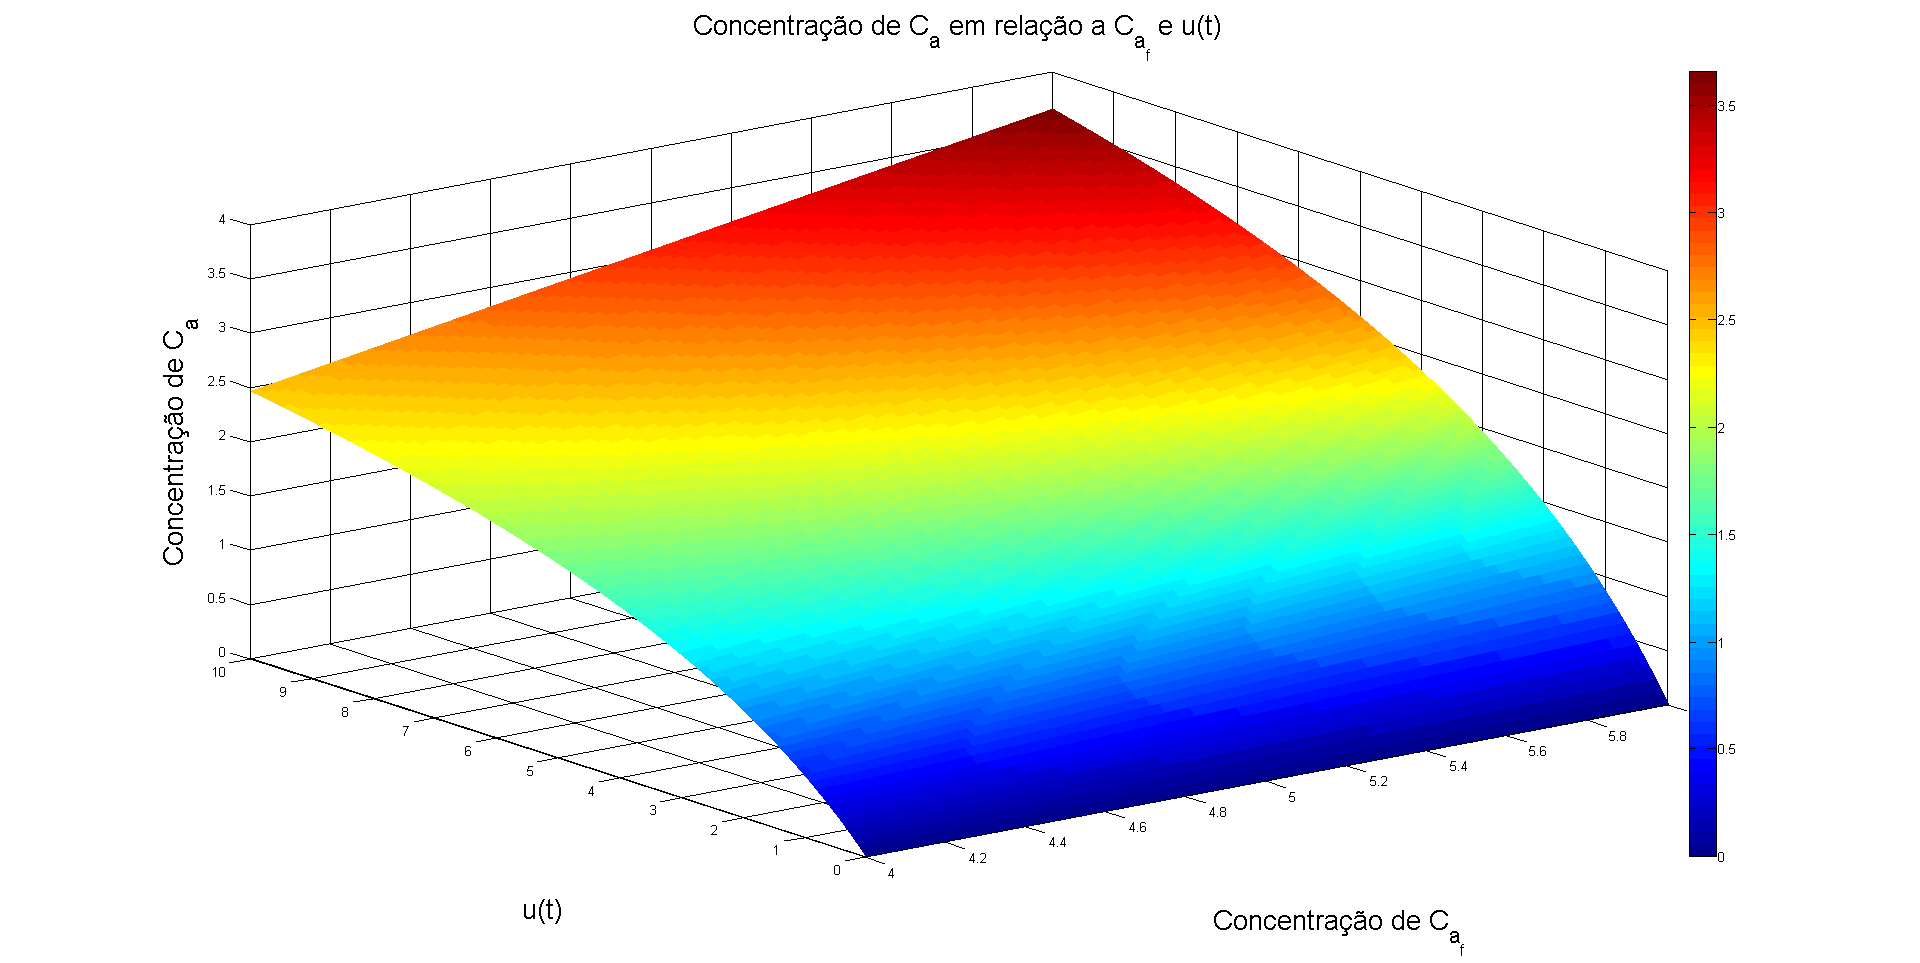
\includegraphics[width=1\textwidth]{Imagens/CAFxUxCA.png}
  \caption{Concentração de \( C_a \) variando u(t) e \( C_{a_f} \)}
  \end{figure}

   \begin{figure}[H]
  \centering
  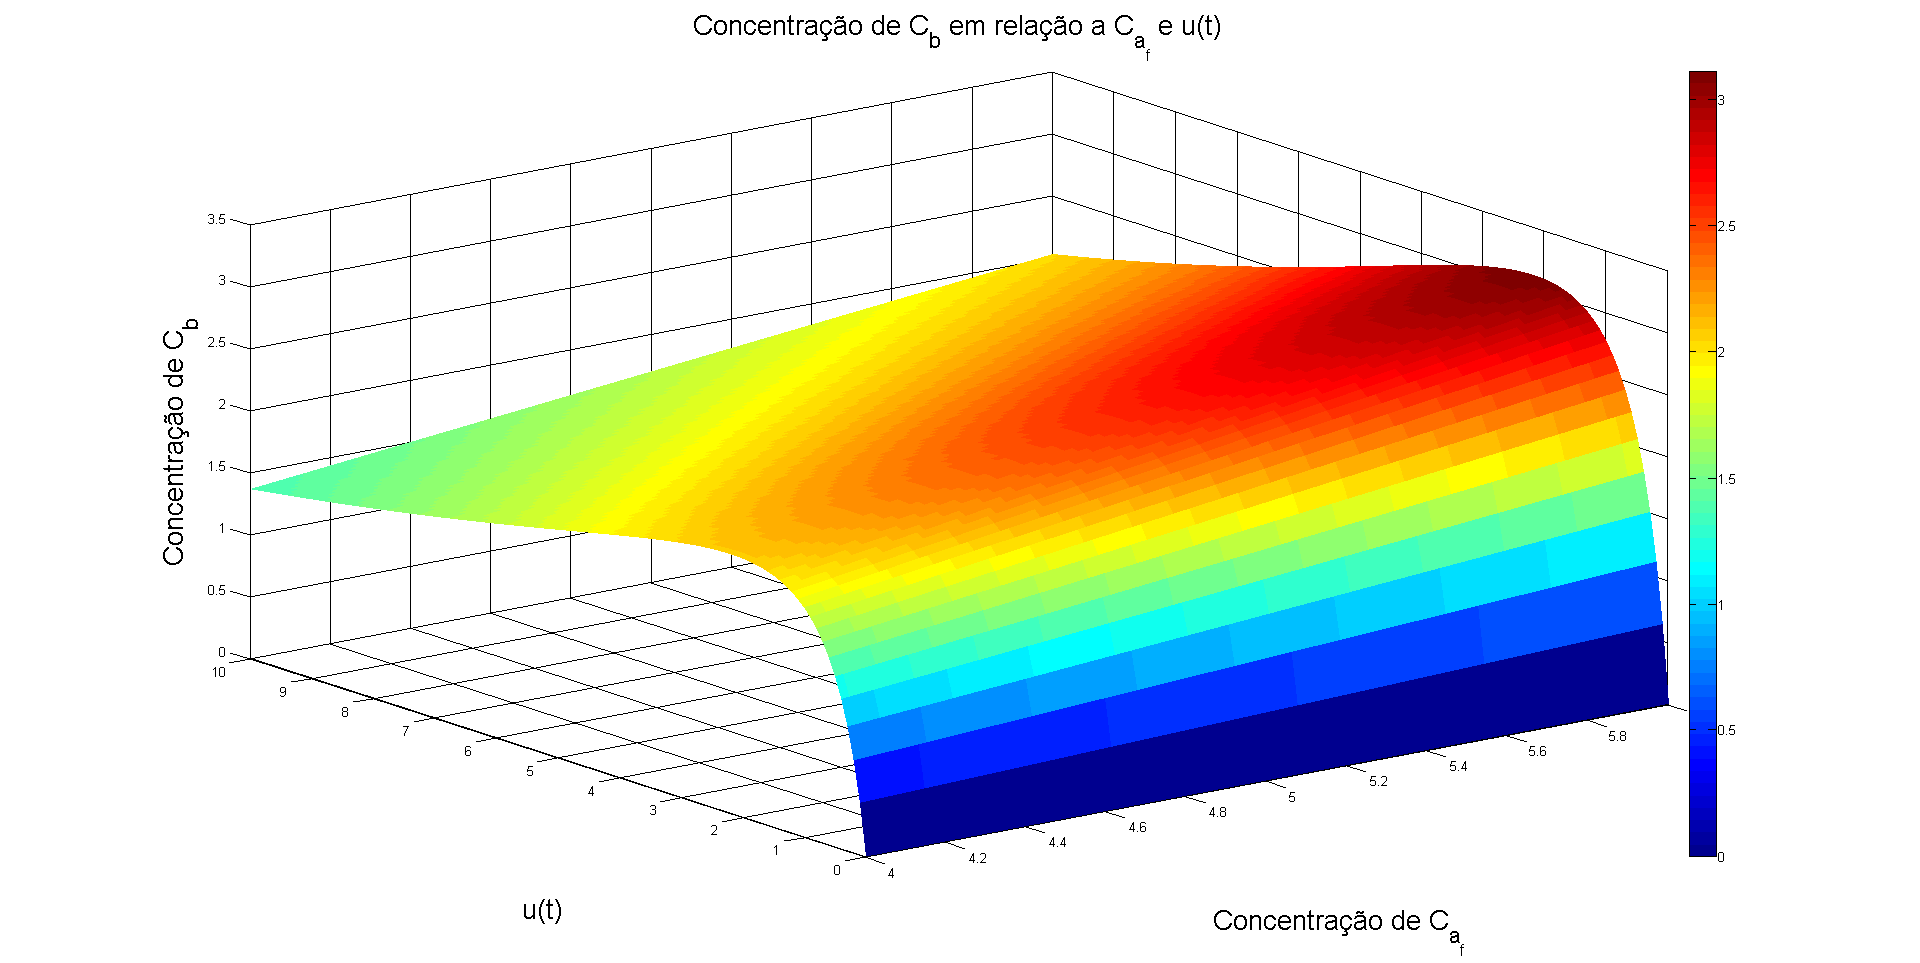
\includegraphics[width=1\textwidth]{Imagens/CAFxUxCB.png}
  \caption{Concentração de \( C_b \) variando u(t) e \( C_{a_f} \)}
  \end{figure}

  Os gráficos acima apresentam a família de pontos de equilíbrio do sistema de acordo com as entradas de controle \(u(t)\) e \(C_{a_f}\) definidas.
  
\newpage





\section{2) Estudo do Comportamento Dinâmico usando Simulink}

Usando Simulink, estude por simulação o comportamento dinâmico do sistema e verifique os pontos de equilíbrio encontrados no modelo estático. Para o ponto de equilíbrio dado por \( C_{af} = 5.1 \, \text{mol/L} \) e \( u = 1 \, \text{min}^{-1} \), determine a concentração de funcionamento em equilíbrio do produto A (\( C_a \)) e do produto B (\( C_b \)).

A partir das equações 2.2 e 2.3, obtem-se:

\begin{align}
\frac{dC_a}{dt} &= C_a(-k_1-u(t))- k_3 C_a^2 +C_{a_f} u(t)\\
\frac{dC_b}{dt} &= k_1 C_a - k_2 C_b - C_b u(t)\\
\end{align}

Adaptando essas equações para o Simulink, com entradas do ponto de equilíbrio \(u(t) = 1 l/min\) e \(C_{a_f} = 5.1 l/min\), o seguinte modelo é montado:


 \begin{figure}[H]
  \centering
  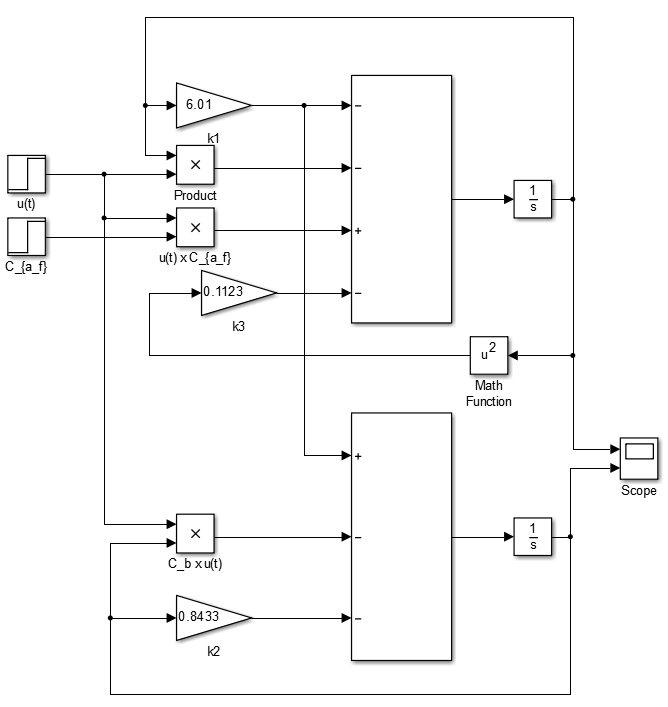
\includegraphics[width=0.7\textwidth]{Imagens/Q2Simu.png}
  \caption{Modelo Simulink dos sistema de equações 2.21 e 2.22}
  \end{figure}


 \begin{figure}[H]
  \centering
  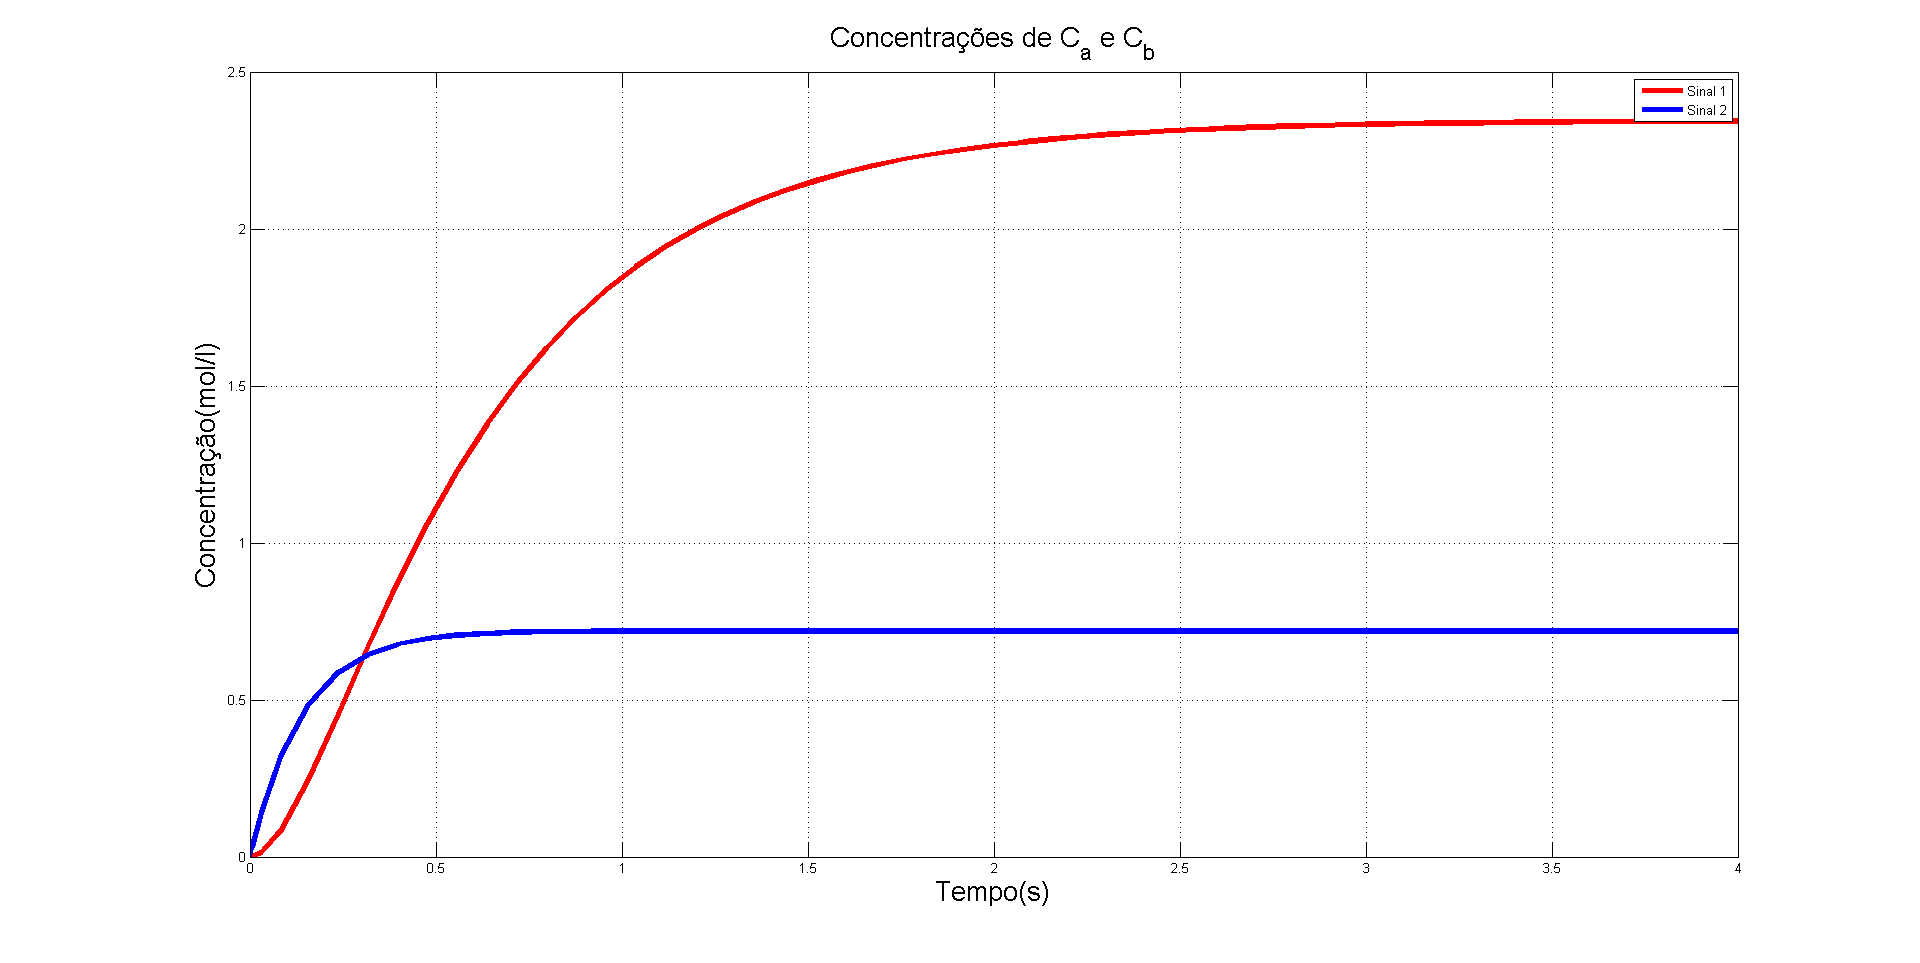
\includegraphics[width=1\textwidth]{Imagens/Q2.png}
  \caption{Resposta às concentrações de $C_a$ e $C_b$}
  \end{figure}

  A análise das concentrações \( C_a \) e \( C_b \) de regime permanente indicam os valores:\\
\begin{align}
 C_a = 0.719 \ \text{mol/L}\\
 C_b = 2.345 \ \text{mol/L}
\end{align}

\newpage

\section{3) Linearização do Sistema}

Para o ponto achado, linearize o sistema encontrando um modelo incremental dinâmico. Desenhe um diagrama de blocos do sistema não linear e do sistema linearizado. Aplique a transformada de Laplace no sistema linearizado e desenhe o diagrama de blocos em domínio “s”.\\

Linearizando o sistema, iniciando pela Equação Diferencial Original da variação da concentração do produto A:

\begin{align}
\frac{dC_a}{dt} &= -k_1 C_a - k_3 C_a^2 + (C_{a_f}-C_a) u(t)\\
\end{align}

Definindo pontos de equilíbrio:

\begin{align}
u(t) = \overline{u} + \Delta{u}\\
C_a = \overline{\mathrm{C}_a} + \Delta{C}_a\\
C_{a_f} = \overline{\mathrm{C}_{a_f}} + \Delta{C}_{a_f}\\
\end{align}

Aplicando os ponto de equilíbrio na Equação Diferencial Original 2.26:

\begin{align}
\frac{dC_a}{dt} &= -k_1 [ \overline{\mathrm{C}_a} + \Delta{C}_a] - k_3 [\overline{\mathrm{C}_a}^2 + \Delta{C}_a^2] - u [\overline{\mathrm{C}_a} + \Delta{C}_a] + u [\overline{\mathrm{C}_{a_f}} + \Delta{C}_{a_f}]\\
\end{align}

Seguindo com a derivação da equação linearizada:

\begin{align}
\frac{dC_a}{dt} &= \frac{\partial C_a}{\partial C_a}[C_a-\overline{\mathrm{C}_a}] + \frac{\partial C_a}{\partial C_{a_f}}[C_{a_f}-\overline{\mathrm{C}_{a_f}}] + \frac{\partial C_a}{\partial u}[u-\overline{u}]
\end{align}

\begin{align}
\Delta\frac{dC_a}{dt} &= \frac{\partial C_a}{\partial C_a}\Delta C_a + \frac{\partial C_a}{\partial C_{a_f}}\Delta C_{a_f} + \frac{\partial C_a}{\partial u}\Delta u
\end{align}

Em que cada componente derivada parcial é:

\begin{align}
\frac{\partial C_a}{\partial C_a} = \frac{\partial [-k_1 C_a - k_3 C_a^2 +u (C_{a_f}-C_a)]}{\partial C_a}\\
\frac{\partial C_a}{\partial C_a} = -k_1-2 k_3 \overline{\mathrm{C}_a} - \overline{u}\\
\frac{\partial C_a}{\partial C_{a_f}} = \frac{\partial [-k_1 C_a - k_3 C_a^2 +u (C_{a_f}-C_a)]}{\partial C_{a_f}}\\
\frac{\partial C_a}{\partial C_{a_f}} = \overline{u}\\
\frac{\partial C_a}{\partial u} = \frac{\partial [-k_1 C_a - k_3 C_a^2 +u (C_{a_f}-C_a)]}{\partial u}\\
\frac{\partial C_a}{\partial u} = \overline{\mathrm{C}_{a_f}} - \overline{\mathrm{C_a}}
\end{align}

Substituindo as derivadas parciais 2.37, 2.39 e 2.41 na equação 2.35, obtem-se:

\begin{align}
\Delta\frac{dC_a}{dt} = (-k_1 - 2 k_3\overline{\mathrm{C_a}}-\overline{u})\Delta C_a + \overline{u}\Delta C_{a_f} + (\overline{\mathrm{C}_{a_f}} - \overline{\mathrm{C_a}})\Delta u
\end{align}

Utilizando os valores já definidos anteriormente no enunciado e nos pontos de equilíbrio encontrados:

\begin{align*}
k_1 &= 6.01 \\
k_2 &= 0.8433 \\
k_3 &= 0.1123 \\
\overline{u} &= 1 \\
\overline{C}_{a_f} &= 5.1 \ \text{mol/L}\\
\overline{C}_a &= 0.719 \ \text{mol/L} \\
\overline{C}_b &= 2.345 \ \text{mol/L}
\end{align*}

\begin{align}
\Delta\frac{dC_a}{dt} = \left(-6.01 - 2 \cdot 0.1123 \cdot 0.719 - 1\right)\Delta C_a + 1 \cdot \Delta C_{a_f} + (5.1 - 0.719)\Delta u \\
\Delta\frac{dC_a}{dt} = \left(-6.01 - 0.1614 - 1\right)\Delta C_a + \Delta C_{a_f} + 4.381\Delta u \\
\Delta\frac{dC_a}{dt} = -7.1714 \Delta C_a + \Delta C_{a_f} + 4.381\Delta u \\
\end{align}

Continuando a linearização do sistema, agora pela Equação Diferencial Original da variação da concentração do produto B:

\begin{align}
\frac{dC_b}{dt} &= k_1 C_a - k_2 C_b - C_b u(t)\\
\end{align}

\begin{align}
u(t) = \overline{u} + \Delta{u}\\
C_a = \overline{\mathrm{C}_a} + \Delta{C}_a\\
C_b = \overline{\mathrm{C_b}} + \Delta{C_b}
\end{align}

\begin{align}
\Delta\frac{dC_b}{dt} &= k_1 [\overline{\mathrm{C}_a} + \Delta{C}_a] - k_2 [\overline{\mathrm{C_b}} + \Delta{C_b}] - [\overline{\mathrm{C_b}} + \Delta{C_b}][\overline{u} + \Delta{u}]
\end{align}

\begin{align}
\Delta\frac{dC_b}{dt} &= \frac{\partial C_b}{\partial C_a}\Delta C_a + \frac{\partial C_b}{\partial C_b}\Delta C_b + \frac{\partial C_b}{\partial u}\Delta u
\end{align}

Dessa forma, cada parcial é: \\

\begin{align}
\frac{\partial C_b}{\partial C_a} = k_1\\
\frac{\partial C_b}{\partial C_b} = -k_2 - u\\
\frac{\partial C_b}{\partial u} = -C_b\\
\Delta\frac{dC_b}{dt} = k_1\Delta C_a + (-k_2-u)\Delta C_b - C_b\Delta u
\end{align}

Como \(C_b\) e \(u\) encontrados na equação acima devem estar no ponto de operação, iguala-se aos valores constantes.


\begin{align}
\Delta\frac{dC_b}{dt} = k_1\Delta C_a + (-k_2-\overline{u})\Delta C_b - \overline{\mathrm{C_b}}\Delta u
\end{align}

Substituindo os valores encontrados anteriormente \(k_1 = 6.01\), \(k_2 = 0.8433\), \(k_3 = 0.1123\) e \(\overline{\mathrm{C_b}} = 2.345\ \text{mol/L}\):

\begin{align}
\Delta\frac{dC_b}{dt} = 6.01 \Delta C_a + (-0.8433-1)\Delta C_b - 2.354 \Delta u\\
\Delta\frac{dC_b}{dt} = 6.01 \Delta C_a -1.8433\Delta C_b - 2.354 \Delta u
\end{align}

O sistema de equações lineares resultantes é descrito por:

\begin{align}
\Delta\frac{dC_a}{dt} = -7.171 \Delta C_a + \Delta C_{a_f} + 4.381\Delta u \\
\Delta\frac{dC_b}{dt} = 6.01 \Delta C_a -1.843\Delta C_b - 2.354 \Delta u\\
\end{align}

O diagrama de blocos do sistema não linearizado é:

 \begin{figure}[H]
  \centering
  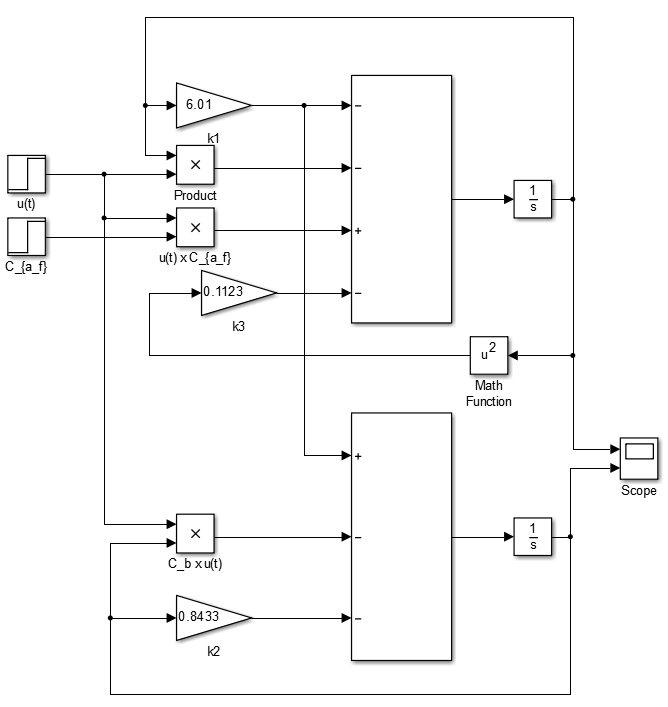
\includegraphics[width=0.7\textwidth]{Imagens/Q2Simu.png}
  \caption{Modelo Simulink do sistema não linearizado}
  \end{figure}

O diagrama de blocos do sistema linearizado é:

 \begin{figure}[H]
  \centering
  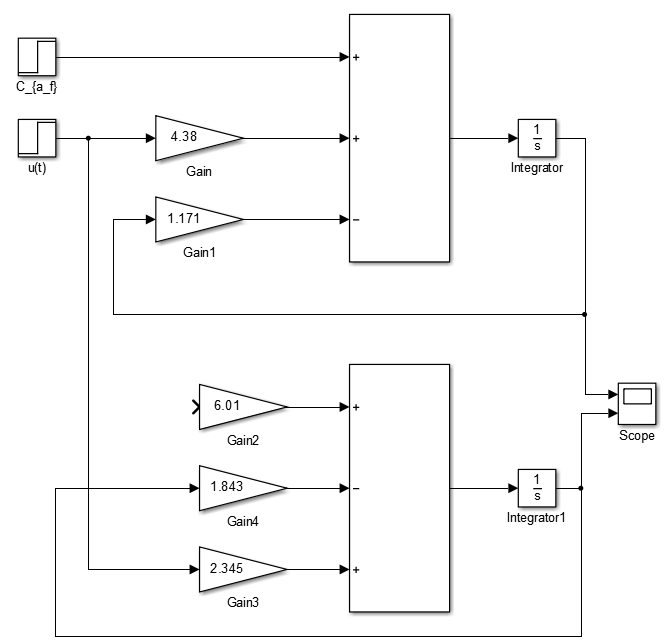
\includegraphics[width=0.7\textwidth]{Imagens/Q3Simu.png}
  \caption{Modelo Simulink do sistema linearizado}
  \end{figure}


Aplicando a transformada de Laplace na equação linearizada de \(C_a\):
\begin{align}
s \Delta C_a(s) = -7.171 \Delta C_a(s) + \Delta C_{a_f}(s) + 4.381 \Delta u(s)
\end{align}

Resolvendo para \(\Delta C_a(s)\):
\begin{align}
s \Delta C_a(s) + 7.171 \Delta C_a(s) &= \Delta C_{a_f}(s) + 4.381 \Delta u(s) \\
(s + 7.171) \Delta C_a(s) &= \Delta C_{a_f}(s) + 4.381 \Delta u(s) \\
\Delta C_a(s) &= \frac{\Delta C_{a_f}(s) + 4.381 \Delta u(s)}{s + 7.171}
\end{align}

Aplicando a transformada de Laplace na equação linearizada de \(C_b\):

Aplicando a transformada de Laplace:
\begin{align}
s \Delta C_b(s) = 6.01 \Delta C_a(s) - 1.843 \Delta C_b(s) - 2.354 \Delta u(s)
\end{align}

Resolvendo para \(\Delta C_b(s)\):
\begin{align}
s \Delta C_b(s) + 1.843 \Delta C_b(s) &= 6.01 \Delta C_a(s) - 2.354 \Delta u(s) \\
(s + 1.843) \Delta C_b(s) &= 6.01 \Delta C_a(s) - 2.354 \Delta u(s) \\
\Delta C_b(s) &= \frac{6.01 \Delta C_a(s) - 2.354 \Delta u(s)}{s + 1.843}
\end{align}

Portanto, o diagrma de blocos para o sistema linearizado e no domínio da frequência é:

\begin{figure}[H]
  \centering
  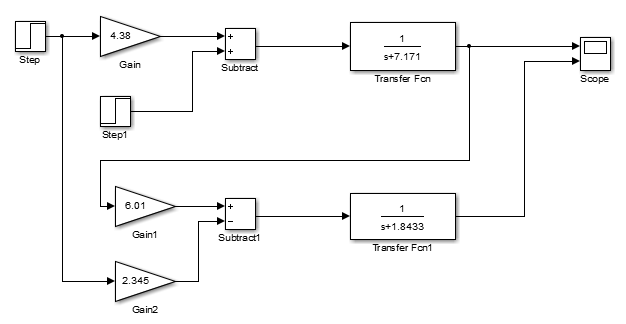
\includegraphics[width=0.7\textwidth]{Imagens/Q3SimuS.png}
  \caption{Modelo Simulink do sistema linearizado no domínio da frequência}
  \end{figure}









\newpage

\section{4) Funções de Transferência}

Para determinar a concentração do produto \(A\), utilizamos o seguinte diagrama de blocos:

\[
\Delta C_a(s) = G_1 \Delta U' + \Delta C_{af}
\]

Substituindo os valores, temos:

\[
\Delta C_a(s) = G_1 \cdot 4.38 \Delta U + \Delta C_{af}
\]

Portanto, podemos expressar a equação como:

\[
\Delta C_a(s) = \frac{4.38 \Delta U + \Delta C_{af}}{s + 7.171}
\]

Para a concentração do produto \(B\), o diagrama de blocos nos dá:

\[
\Delta C_b(s) = G_2 \Delta C' - \Delta U''_b
\]

Inserindo os valores apropriados, temos:

\[
\Delta C_b(s) = G_2 \cdot 6.01 \Delta C - 2.345 \Delta U_b
\]

Assim, a equação fica:

\[
\Delta C_b(s) = \frac{26.01 \Delta C - 2.345 \Delta U_b}{s + 1.8433}
\]

Consequentemente, as equações para as concentrações dos produtos \(A\) e \(B\) são:

\[
\Delta C_a(s) = \frac{\Delta C_{af} + 4.38 \Delta U}{s + 7.171}
\]

\[
\Delta C_b(s) = \frac{\Delta C_{af} - 2.345 \Delta U_b}{6.01 (s + 1.8433)}
\]

Até este ponto, observamos que \(\Delta C_a(s)\) é uma função da variável manipulada \(\Delta U\) e da principal perturbação \(\Delta C_{af}\). No entanto, para que \(\Delta C_b(s)\) também dependa dessas variáveis, precisamos fazer algumas manipulações adicionais.

Substituindo \(\Delta C_a(s)\) na equação (7), obtemos:

\[
\Delta C_b(s) = \frac{4.38 \Delta U + \Delta C_{af} - 2.345 \Delta U_b}{(s + 1.8433)(s + 7.171)}
\]

Ao simplificar, chegamos a:

\[
\Delta C_b(s) = \frac{(4.38 \Delta U + \Delta C_{af} - 2.345 \Delta U_b)}{(s + 1.8433)(s + 7.171)}
\]

Dessa forma, as quatro funções de transferência são:

\[
\frac{\Delta C}{\Delta C_{af}} = \frac{1}{s + 7.171}
\]

\[
\frac{\Delta C}{\Delta U} = \frac{4.38}{s + 7.171}
\]

\[
\frac{\Delta C}{\Delta C_b} = \frac{6.01}{(s + 1.8433)(s + 7.171)}
\]

\[
\frac{\Delta C}{\Delta U_b} = \frac{-2.345}{(s + 1.8433)(s + 7.171)}
\]

\newpage

\section{5) Simulação e Análise em Matlab}

Usando Simulink, estude por simulação o comportamento deste sistema e compare o comportamento com o do sistema não linear nas proximidades do ponto de equilíbrio. Repita a análise usando MATLAB (código .m). Para a simulação em MATLAB do processo, aproxime as derivadas por \( \frac{dx}{dt} = \frac{1}{T_c}(x(k+1) - x(k)) \), sendo \( T_c \) o tempo de cálculo da aproximação.


Para analisar o comportamento do sistema linearizado em comparação com o sistema não linear, levamos o sistema não linear ao seu ponto de operação. Em seguida, aplicamos pequenas variações nas entradas de ambos os sistemas enquanto monitoramos as saídas.

Utilizando os diagramas de blocos do sistema não linear e do sistema linearizado desenvolvidos anteriormente, aplicamos uma variação de \(0.1 \, \text{l/min}\) em \(u\) e de \(2 \, \text{mol/l}\) em \(C_{af}\).

\begin{figure}[h]
    \centering
    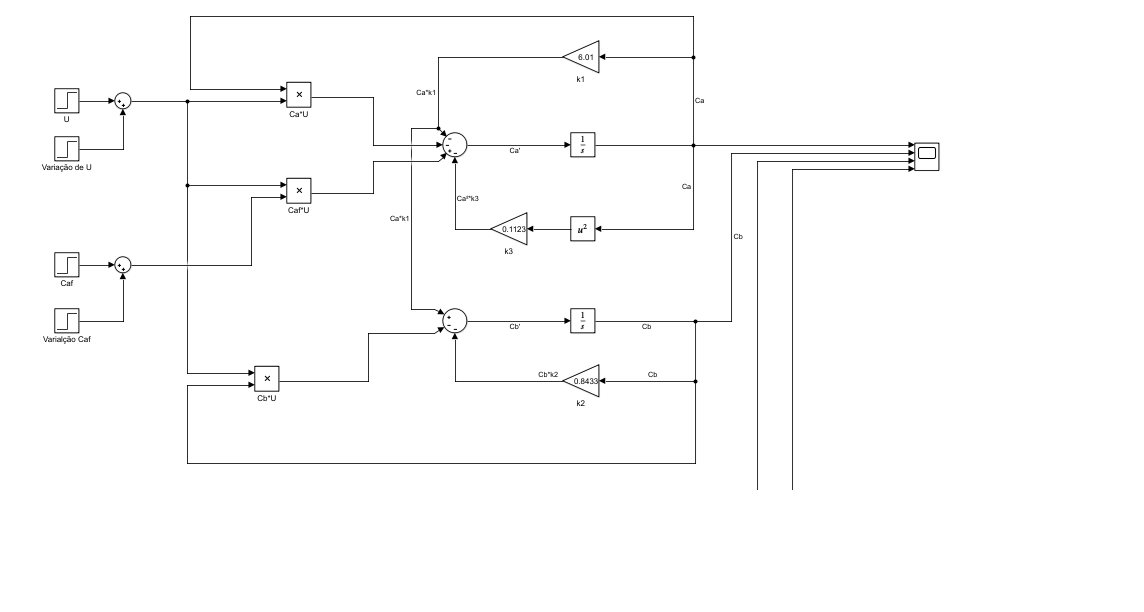
\includegraphics[width=0.9\textwidth]{figura8_1.png}
   % \caption{Comparação entre sistemas linear e não linear}
\end{figure}

\begin{figure}[h]
    \centering
    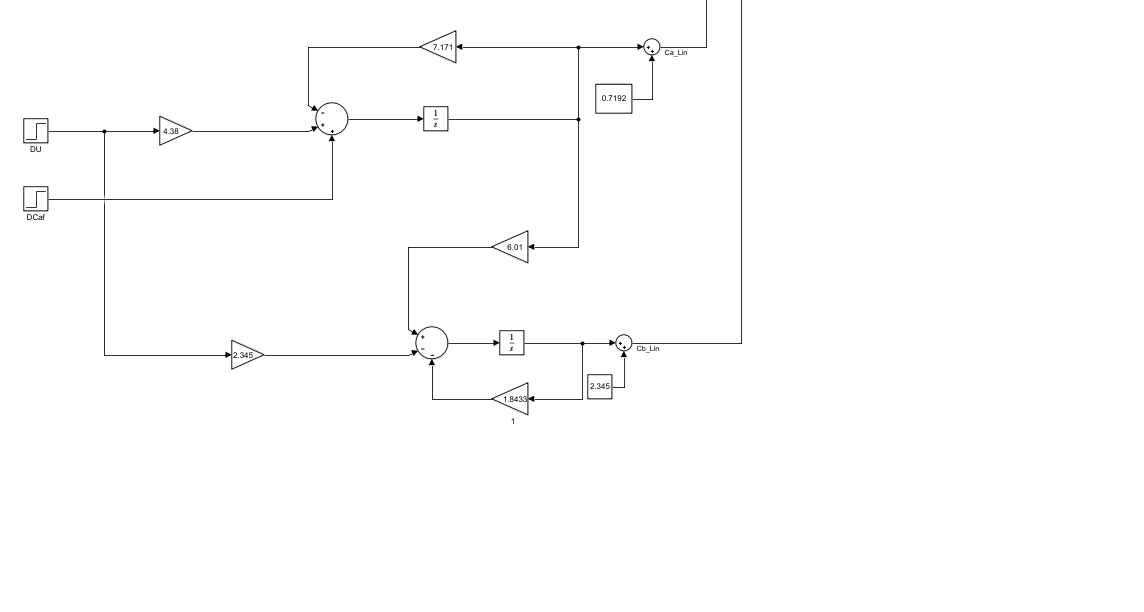
\includegraphics[width=0.9\textwidth]{figura8.png}
    \caption{Comparação entre sistemas linear e não linear}
\end{figure}

A resposta obtida está ilustrada na Figura 9, onde comparamos as respostas dos sistemas linear e não linear utilizando o Simulink.

\begin{figure}[h]
    \centering
    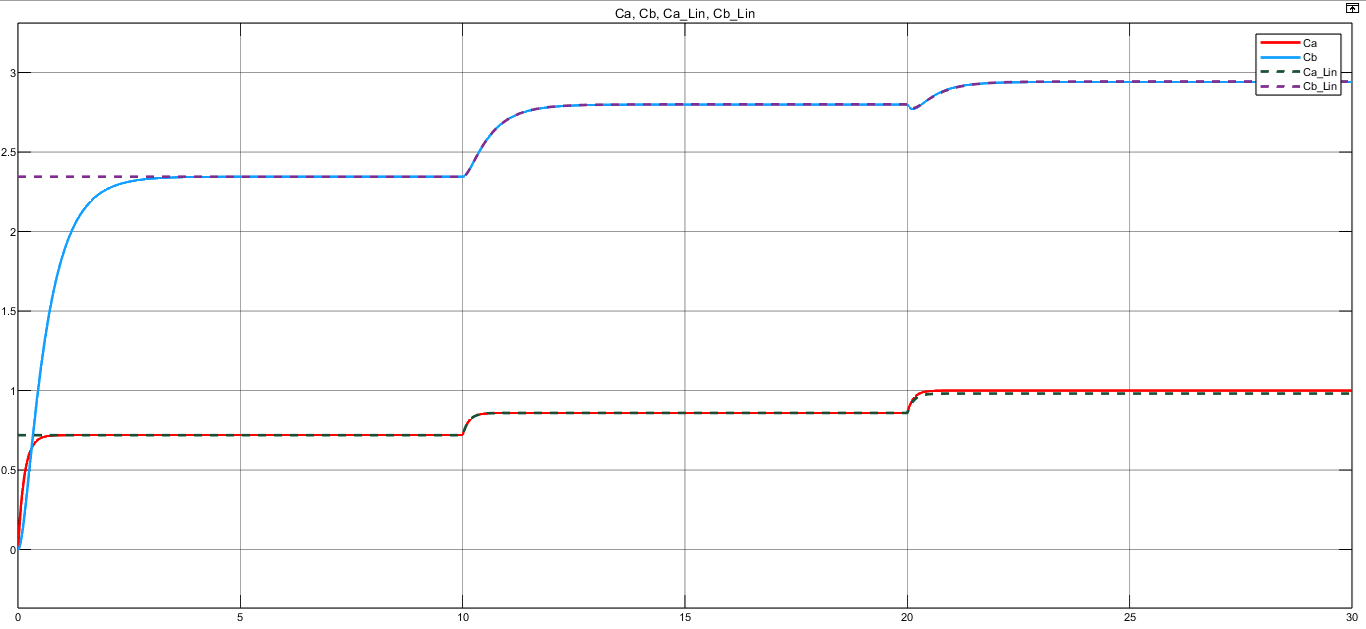
\includegraphics[width=0.8\textwidth]{figura9.png}
    \caption{Respostas dos sistemas linear e não linear (Simulink)}
\end{figure}

Observamos que, para pequenas variações nas entradas, ambos os sistemas convergem para valores similares. No entanto, ao aumentar significativamente a variação, os comportamentos dos sistemas se tornam distintos.

Para a simulação por meio de código, primeiramente determinamos o intervalo de tempo entre as amostras (\(T_c\)) para implementar um método de cálculo numérico, como o método de Euler. Para isso, utilizamos o tempo de acomodação na faixa de 5%.

Vamos analisar as respostas dos sistemas linearizado e não linear:

\begin{figure}[h]
    \centering
    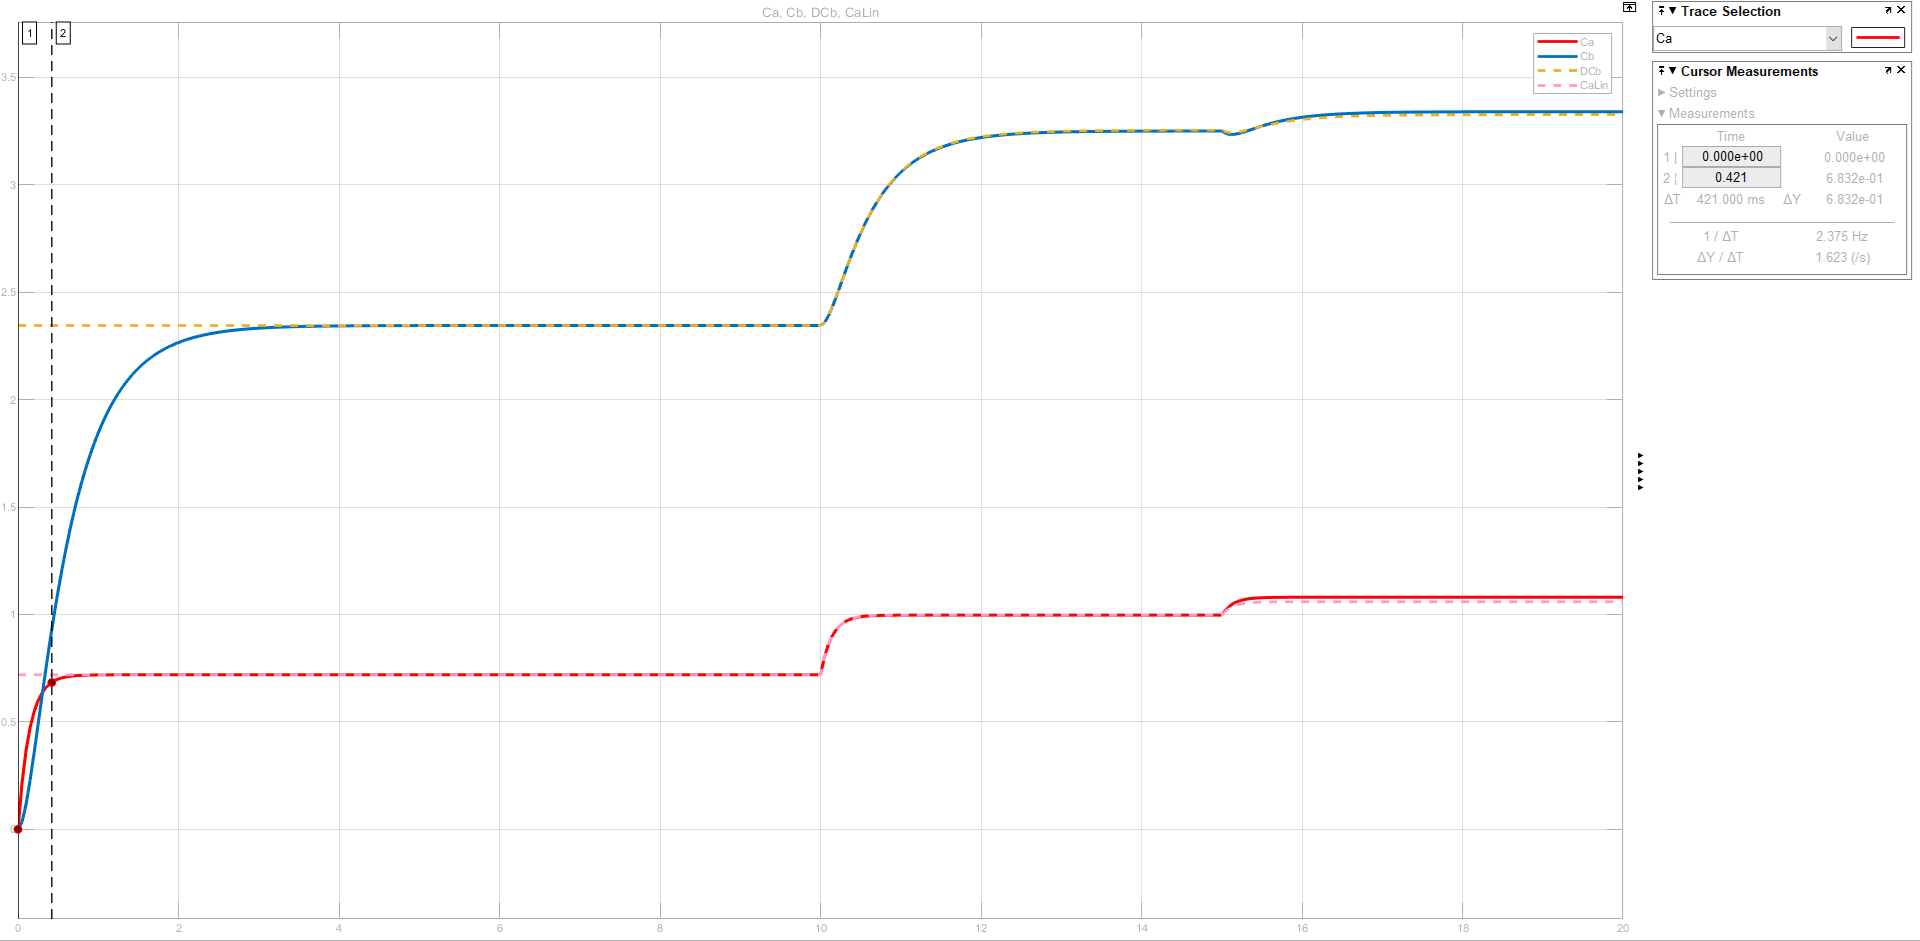
\includegraphics[width=0.8\textwidth]{figura10.png}
    \caption{Tempo de assentamento de \(C_a\)}
\end{figure}

\begin{figure}[h]
    \centering
    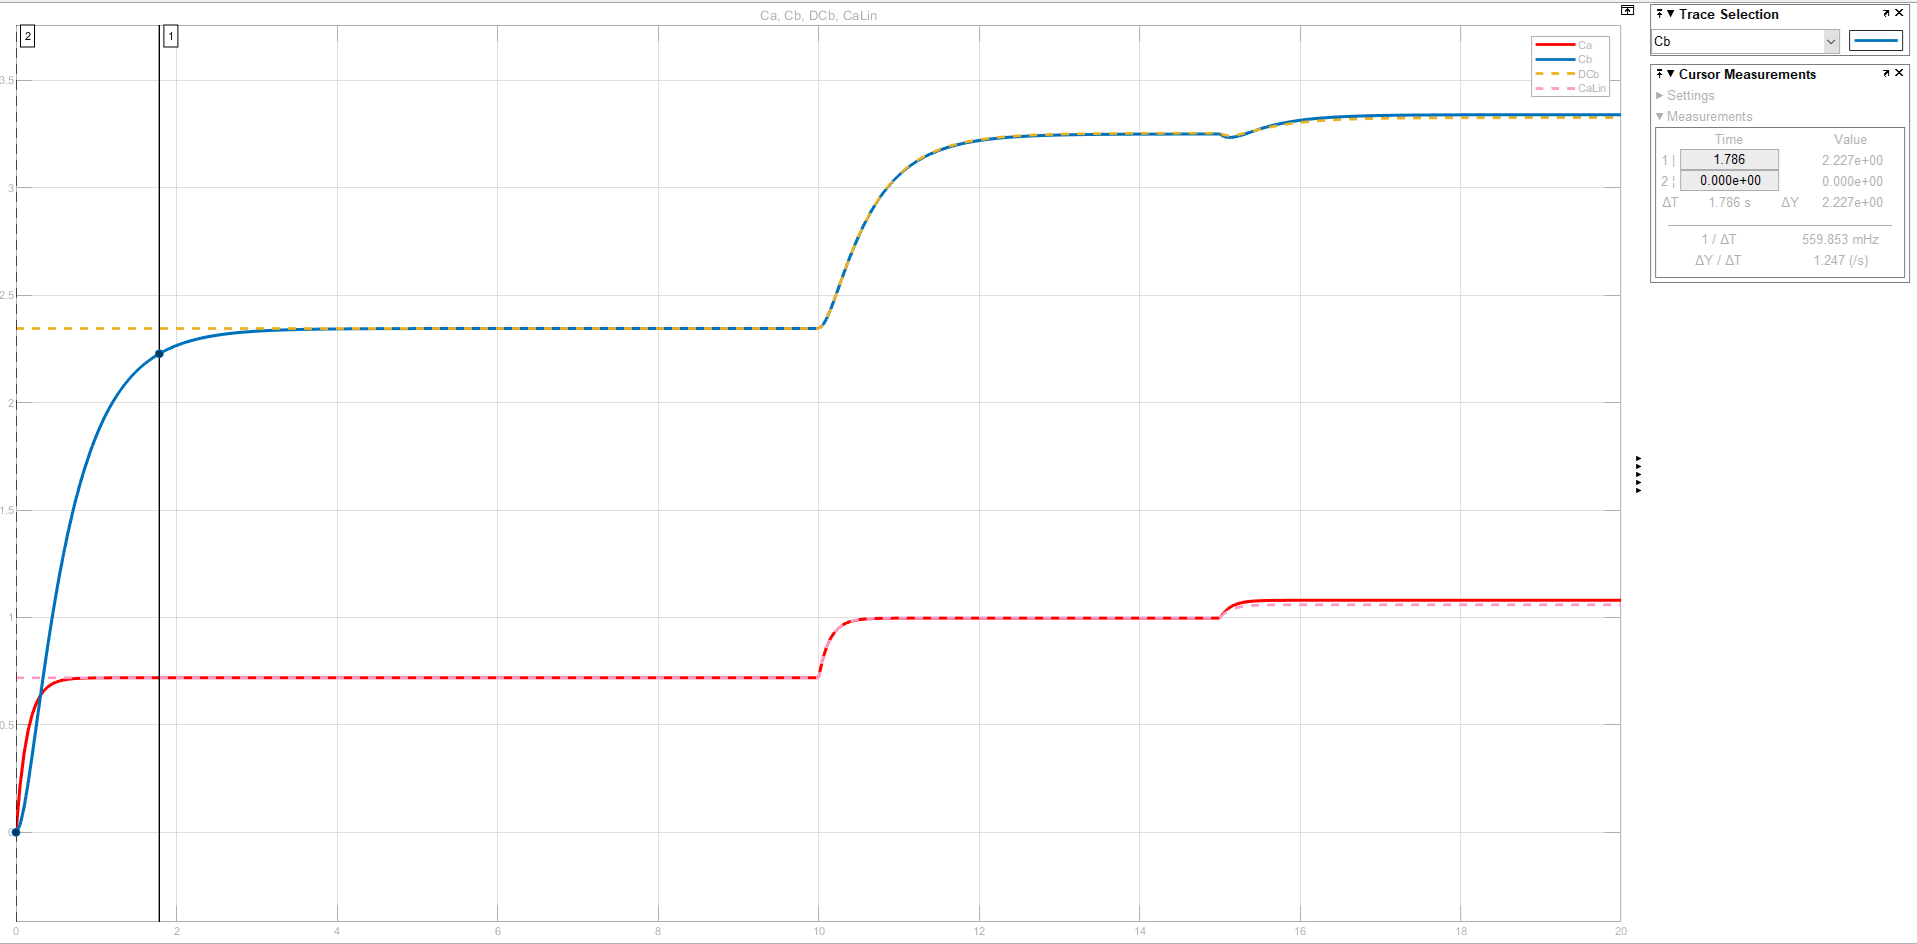
\includegraphics[width=0.8\textwidth]{figura11.png}
    \caption{Tempo de assentamento de \(C_b\)}
\end{figure}

Com base nas respostas dos sistemas não linear e linearizado, obtemos os seguintes tempos de assentamento:

\[
t_{a \rightarrow 5\%} = 0.421 \, s
\]

\[
t_{b \rightarrow 5\%} = 1.786 \, s
\]

Utilizando o menor tempo de assentamento, determinamos o tempo de amostragem \(T_c\) da seguinte maneira:

\[
T_c \leq \frac{t_{5\%}}{20} \approx \frac{0.421}{20} \approx 0.02 \, s
\]

Para o sistema linear, utilizamos a aproximação dada pelo enunciado:

\[
\frac{dx}{dt} \approx \frac{x_{k+1} - x_k}{T_c}
\]

As equações resultantes são:

\[
\Delta C_a = -7.171 \Delta C_a + \Delta C_{af} + 4.38 \Delta u
\]

\[
\Delta C_b = 6.01 \Delta C_a - 1.8433 \Delta C_b - 2.345 \Delta u
\]

Implementando isso no MATLAB, temos:

\begin{lstlisting}[language=Matlab, caption={Exemplo de código MATLAB}, label={lst:matlab}]


close all
clear
clc


k1 = 6.01;
k2 = 0.8433;
k3 = 0.1123;
u = 1;
Caf = 5.1;

% Sistema nao Linear
Tc = 0.02; % tempo de amostragem em segundos
Tsim = 10; % tempo de simulacao em segundos
nit = round(Tsim / Tc); % numero de iteracoes
Ca = zeros(1, nit);
Cb = zeros(1, nit);

% configuracao do grafico
figure
xlabel('Tempo (s)');
ylabel('concentracao (mol/l)');
title('Sistema de Controle com equacao de diferencas');
grid on
pause(1);

% Laco de Controle
for k = 2:nit + 1
    Ca(k) = (-k1 * Ca(k - 1) - u * Ca(k - 1) - k3 * (Ca(k - 1)^2) + Caf * u) * Tc + Ca(k - 1);
    Cb(k) = (k1 * Ca(k - 1) - k2 * Cb(k - 1) - Cb(k - 1) * u) * Tc + Cb(k - 1);
    pause(Tc);
end

% Plot do grafico
plot(0:1:500, Ca);
hold on;
plot(0:1:500, Cb);
\end{lstlisting}

Através deste código, obtemos o seguinte gráfico:

\begin{figure}[h]
\centering
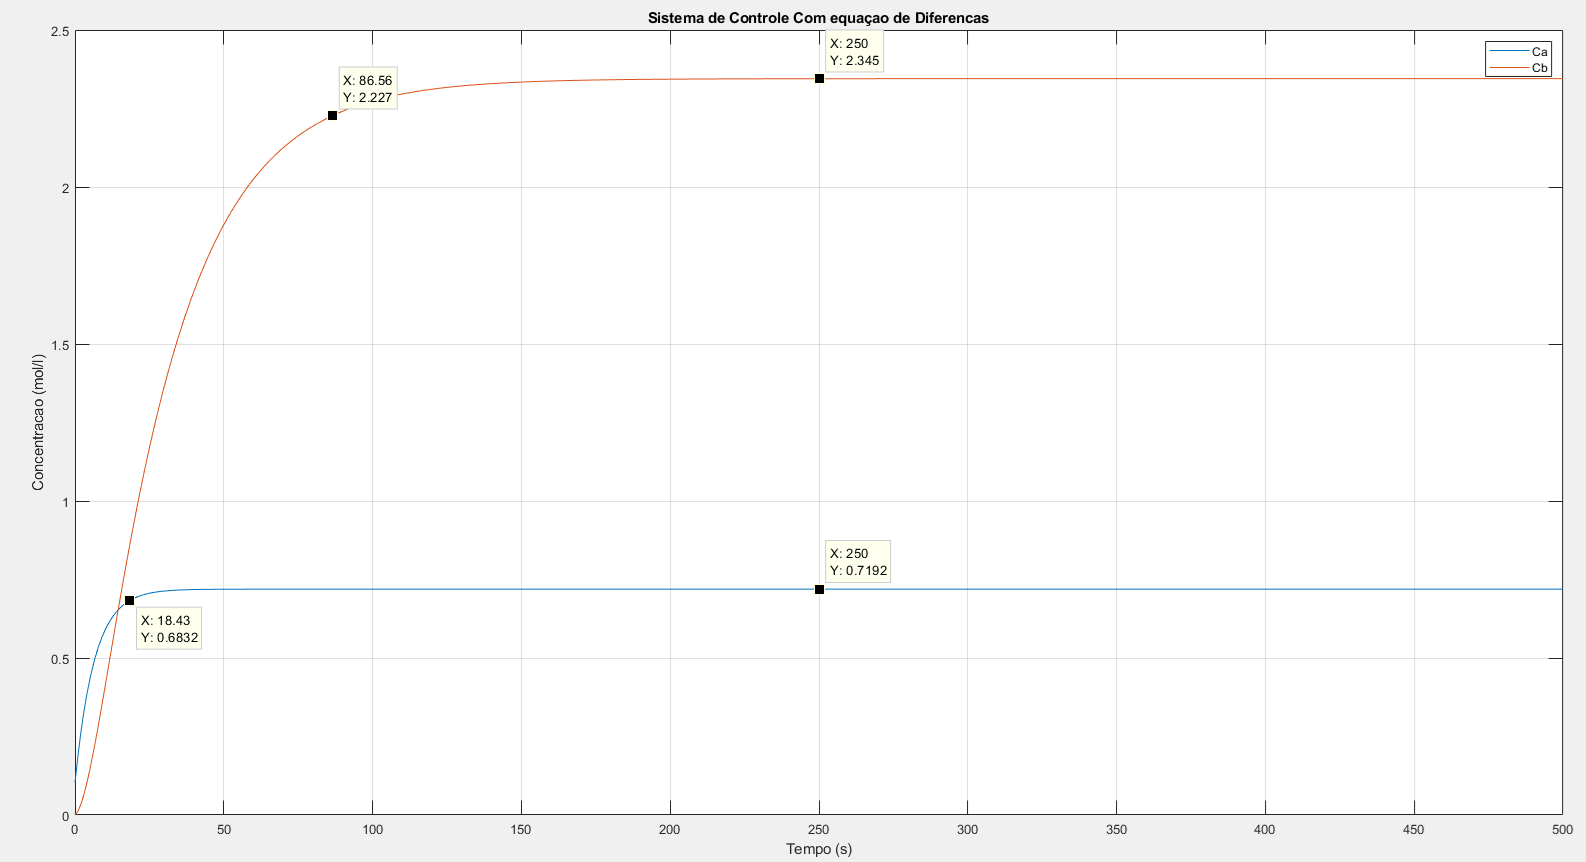
\includegraphics[width=0.8\textwidth]{figura12.png}
\caption{Resposta do sistema linear (Por código)}
\end{figure}

Para o sistema linear, utilizamos a aproximação dada pelo enunciado:

\[
\frac{dx}{dt} \approx \frac{x_{k+1} - x_k}{T_c}
\]

As equações resultantes são:

\[
\Delta C_a = -7.171 \Delta C_a + \Delta C_{af} + 4.38 \Delta u
\]

\[
\Delta C_b = 6.01 \Delta C_a - 1.8433 \Delta C_b - 2.345 \Delta u
\]

Implementando isso no MATLAB, temos:
\begin{lstlisting}[language=Matlab, caption={Exemplo de codigo MATLAB}, label={lst:matlab}]

close all
clear
clc

% Inicializacao das variaveis
u = 1;
Caf = 5.1;

% Sistema Linear
Tc = 0.02; % tempo de amostragem em segundos
Tsim = 10; % tempo de simulacao em segundos
nit = round(Tsim / Tc); % numero de iteracoes
Ca = zeros(1, nit);
Cb = zeros(1, nit);

% Configuracao do grafico
figure
xlabel('Tempo (s)');
ylabel('Concentracao (mol/l)');
title('Sistema de Controle com Equacao de Diferencas');
grid on
pause(1);

% Laco de Controle
for k = 2:nit + 1
    Ca(k) = (-7.171 * Ca(k - 1) + Caf + 4.38 * u) * Tc + Ca(k - 1);
    Cb(k) = (6.01 * Ca(k - 1) - 1.8433 * Cb(k - 1) - 2.345 * u) * Tc + Cb(k - 1);
    pause(Tc);
end

% Plot do grafico
plot(0:1:500, Ca);
hold on;
plot(0:1:500, Cb);

\end{lstlisting}

Através deste código, obtemos o seguinte gráfico:

\begin{figure}[h]
\centering
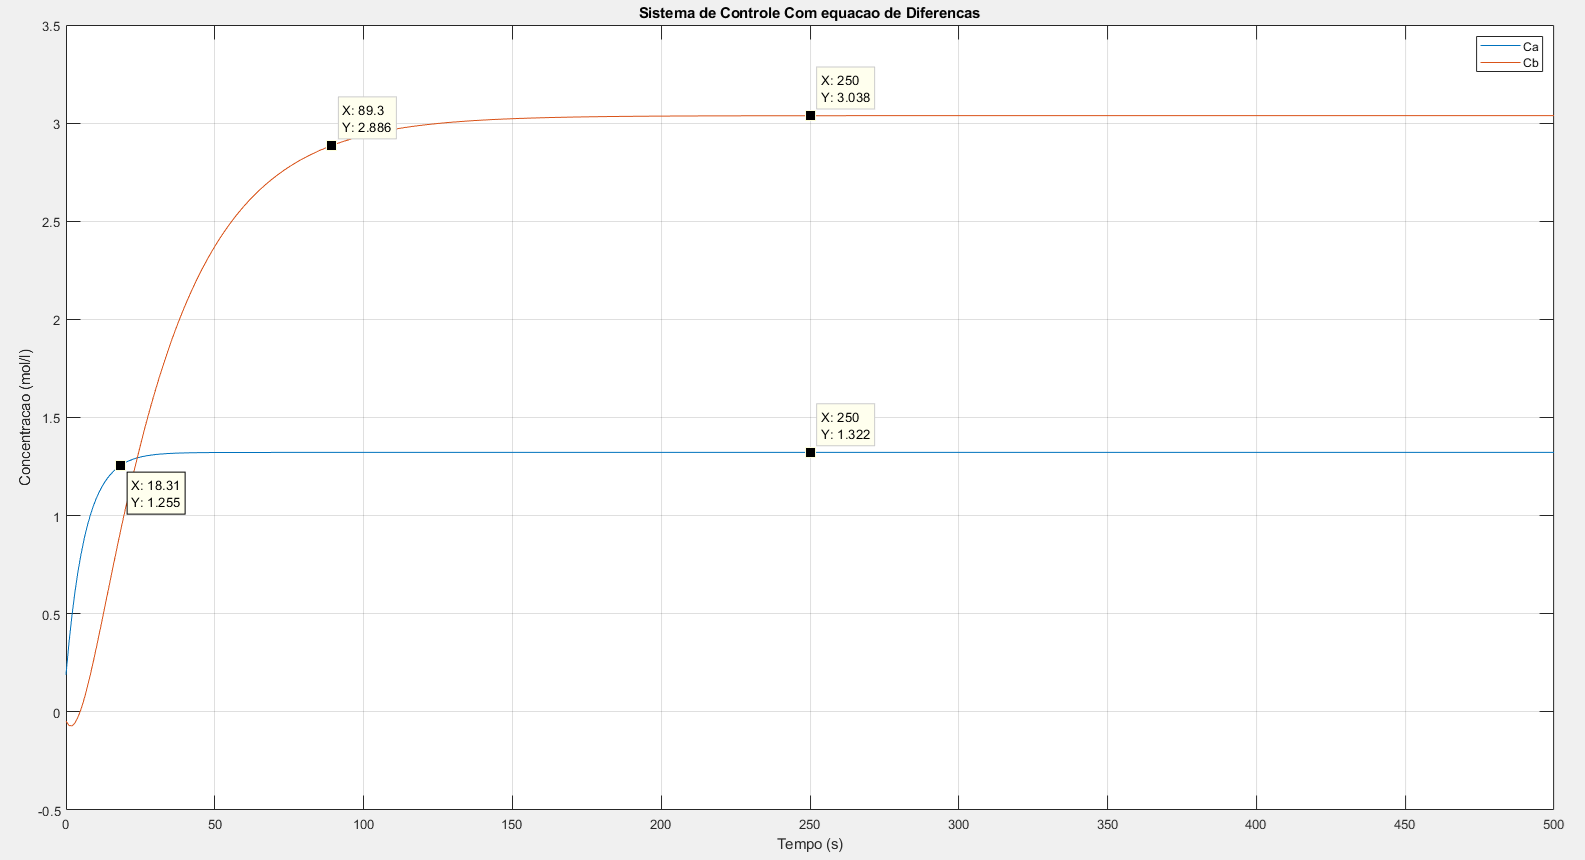
\includegraphics[width=0.8\textwidth]{figura13.png}
\caption{Resposta do sistema linear (Por código)}
\end{figure}



\newpage

\section{6) Projeto de Controle PI}

Realizando experimentos com o modelo não linear nas proximidades do ponto de equilíbrio, obtenha um modelo simples de primeira ordem para as relações entre a variável manipulada e a concentração de B, e a perturbação e a concentração de B. Projete um controle PI contínuo usando a técnica de alocação de polos para obter em malha fechada um sistema com tempo de subida de 5\% da ordem de 1.5 a 1.7 minutos e pico menor que 5\%. Essa especificação deve ser atendida para resposta a seguimentos de degraus de referência de \( C_b \) e perturbações de \( C_{af} \). Use filtro de referência se necessário. Estude o comportamento do sistema sobre o modelo linearizado.


\subsection*{Projeto de Controle PI Contínuo}

Realizando experimentos com o modelo não linear nas proximidades do ponto de equilíbrio, obtemos um modelo simples de primeira ordem para as relações entre a variável manipulada e a concentração de \( B \), e a perturbação e a concentração de \( B \). Projete um controle PI contínuo usando a técnica de alocação de polos para obter em malha fechada um sistema com tempo de subida de 5\% da ordem de 1.5 a 1.7 minutos e pico menor que 5\%. Essa especificação deve ser atendida para resposta a seguimentos de degraus de referência de \( C_b \) e perturbações de \( C_{af} \). Use filtro de referência se necessário. Estude o comportamento do sistema sobre o modelo linearizado.

Primeiro, identificamos a função de transferência aproximada para a concentração de \( B \) em relação à perturbação \( C_{af} \) e à entrada manipulada \( u \):

\[
\Delta C_b(s) = \frac{s+7.171}{6.01} \Delta C_{af}(s) - \frac{s+1.8433}{2.345} \Delta u(s)
\]

Utilizando o modelo linearizado, calculamos os polos e zeros dominantes do sistema.

\subsection*{Obtenção de um Modelo de Primeira Ordem}

Para simplificação, aproximamos o sistema a um modelo de primeira ordem. Calculamos os polos e zeros e ajustamos o ganho para manter a resposta dinâmica desejada.

Primeiro, determinamos o polo \( p \):

\[
p = \frac{4.8}{t_r} = 3
\]

O ganho \( k \) é ajustado para obter o ganho estático desejado:

\[
k = \frac{0.7185}{1.633}
\]

O sistema simplificado é:

\[
G(s) = \frac{0.7185}{s + 1.633}
\]

\subsection*{Projeto do Controlador PI}

Especificações de desempenho:
\begin{itemize}
    \item Tempo de subida de 5\%: 1.5 a 1.7 minutos
    \item Pico menor que 5\%
\end{itemize}

Definimos o controlador PI na forma:

\[
C(s) = k_c \left( 1 + \frac{1}{T_i s} \right) = k_c \frac{T_i s + 1}{T_i s}
\]

Com a função de transferência do sistema em malha fechada sendo:

\[
T(s) = \frac{G(s)C(s)}{1 + G(s)C(s)}
\]

\subsection*{Análise do Polinômio de Malha Fechada}

Verificamos o polinômio de malha fechada para garantir que a quantidade de parâmetros no controlador é suficiente. A função de transferência em malha fechada é dada por:

\[
P_{mf}(s) = (s + p)(s + \alpha) + k (s + \beta)
\]

Para as especificações desejadas, definimos o polinômio de malha fechada desejado com raízes iguais e reais:

\[
P_d(s) = (s + \omega_n)^2 = s^2 + 2\zeta \omega_n s + \omega_n^2
\]

Com \( \zeta = 1 \) e \( \omega_n = \frac{4.8}{t_r} \):

\[
P_d(s) = s^2 + 6s + 9
\]

Igualamos os coeficientes para obter os parâmetros do controlador:

\[
1.175k_c - 0.2898k_c \cdot z_c + 1.633 = 6
\]

\[
1.175k_c \cdot z_c = 9
\]

Resolvendo o sistema, obtemos:

\[
k_c = 1.85162
\]

\[
z_c = 1.91627
\]

Portanto, o controlador PI desenvolvido é:

\[
C(s) = 1.85162 \frac{s + 1.91627}{s}
\]

Simplificando:

\[
C(s) = 1.85162 \left(1 + \frac{1.91627}{s}\right) = 1.85162s + 3.54820
\]

\subsection*{Análise da Resposta do Sistema}

Analisando a resposta do sistema em relação à referência:

\[
Y(s) = \frac{C(s)G(s)}{1 + C(s)G(s)}R(s)
\]

Substituindo \( C(s) \) e \( G(s) \):

\[
Y(s) = \frac{(1.85162s + 3.54820)\left(\frac{0.7185}{s + 1.633}\right)}{1 + (1.85162s + 3.54820)\left(\frac{0.7185}{s + 1.633}\right)}R(s)
\]

\[
Y(s) = \frac{(1.85162s + 3.54820)0.7185}{(s + 1.633) + (1.85162s + 3.54820)0.7185}R(s)
\]

\[
Y(s) = \frac{1.333s + 2.551}{s^2 + 4.05s + 4.8}R(s)
\]

Observa-se um zero no semiplano direito, gerando assim uma fase não mínima. Introduzimos um filtro de referência para cancelar o efeito do zero dominante:

\[
F_r(s) = \frac{1.91627}{s + 1.91627}
\]

Introduzindo o filtro desenvolvido, obtemos a resposta desejada. O comportamento do sistema linearizado com controlador mais o filtro de referência apresenta um sobressinal reduzido e o tempo de acomodação permanece dentro do intervalo desejado.

\begin{figure}[h]
\centering
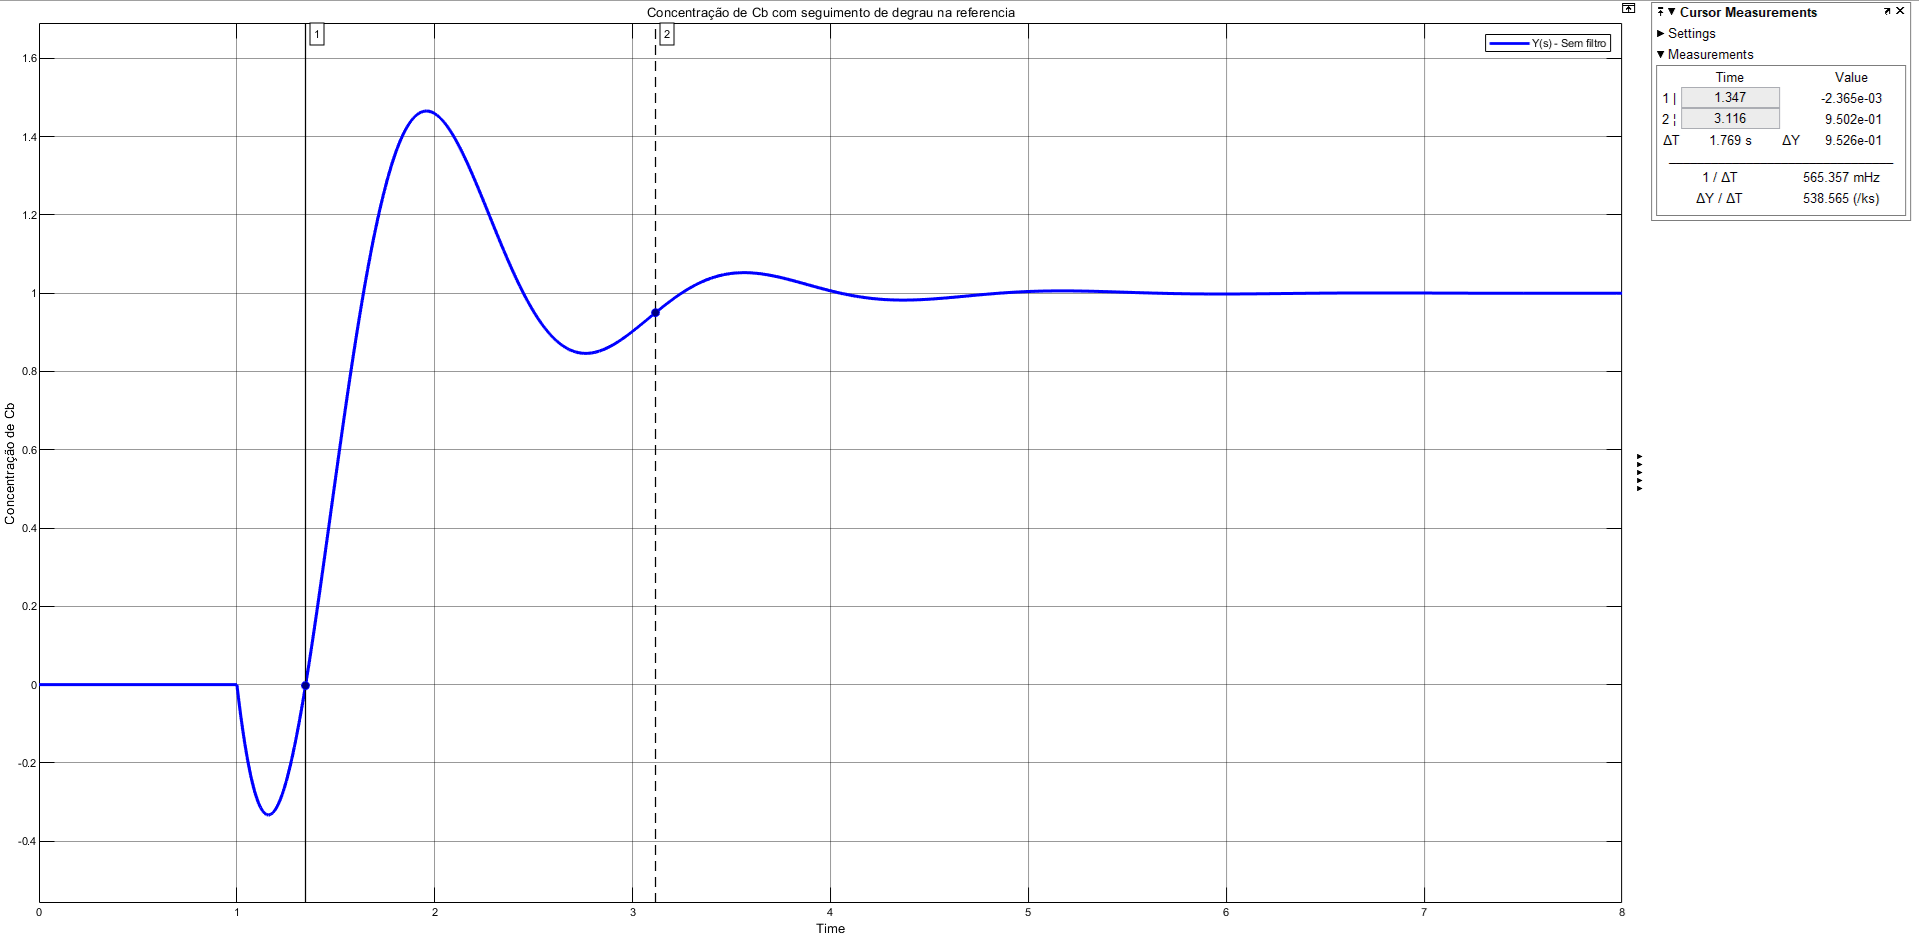
\includegraphics[width=0.8\textwidth]{figura14.png}
\caption{Comportamento do sistema linearizado com controlador tendo um degrau na entrada}
\end{figure}

\begin{figure}[h]
\centering
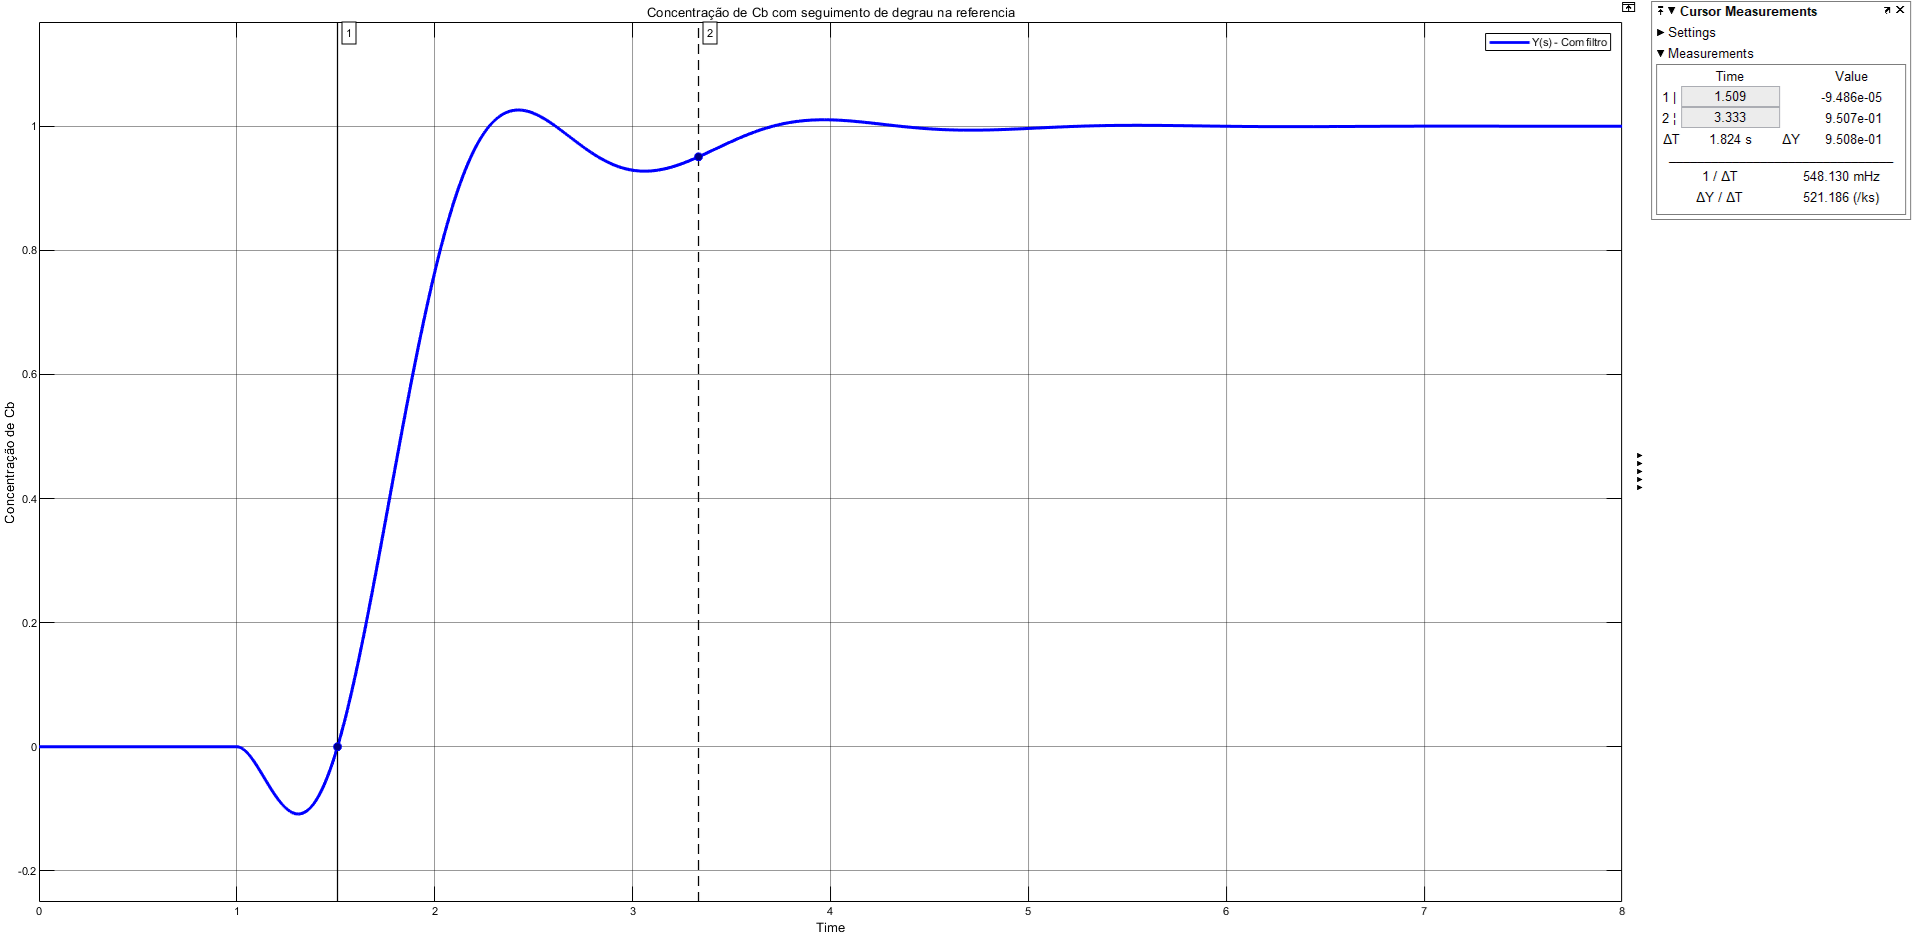
\includegraphics[width=0.8\textwidth]{figura15.png}
\caption{Comportamento do sistema linearizado com controlador mais o filtro de referência tendo um degrau na entrada}
\end{figure}

\subsection*{Resposta à Perturbação}

Analisamos agora a resposta do sistema para uma perturbação aplicada:

\[
Y(s) = \frac{G(s)}{1 + C(s)G(s)}Q(s)
\]

Substituindo \( G(s) \) e \( C(s) \):

\[
Y(s) = \frac{\frac{0.7412}{s + 1.633}}{1 + (1.85162s + 3.54820)\frac{0.7185}{s + 1.633}}Q(s)
\]

\[
Y(s) = \frac{0.7412}{s + 1.633 + (1.85162s + 3.54820)0.7185}Q(s)
\]

\[
Y(s) = \frac{0.7412}{s^2 + 6s + 9}Q(s)
\]

\begin{figure}[H]
\centering
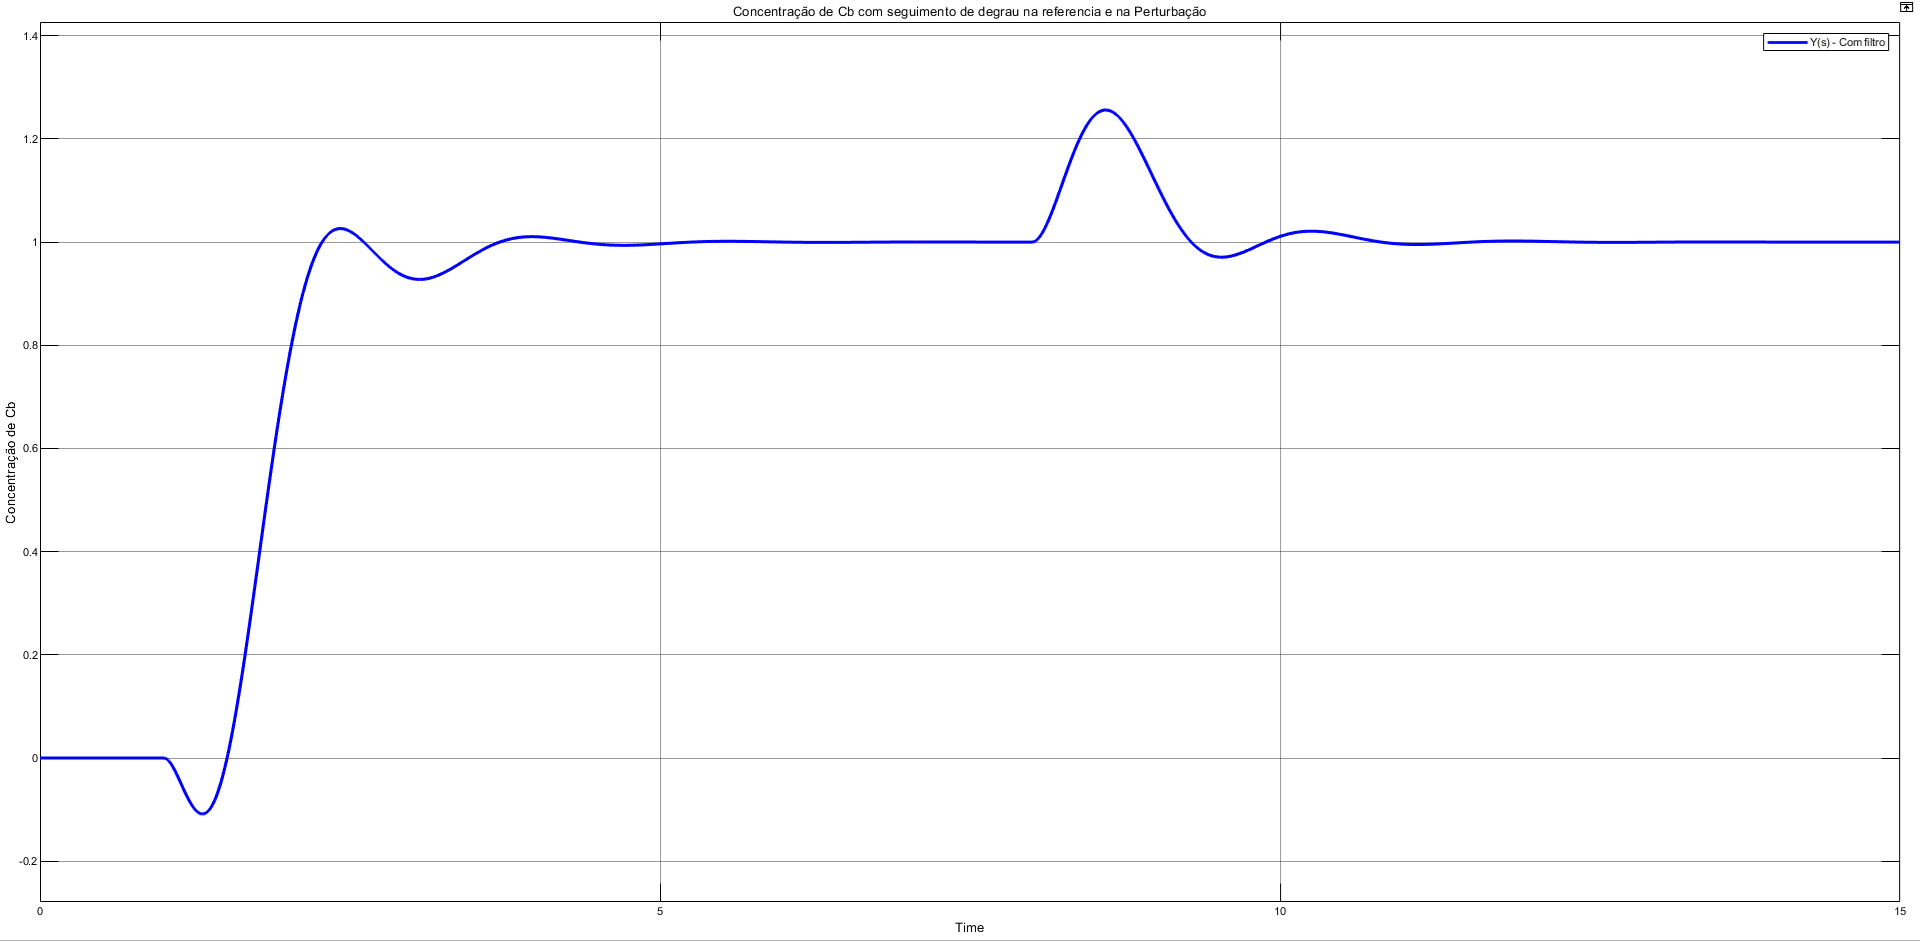
\includegraphics[width=0.8\textwidth]{figura16.png}
\caption{Comportamento do sistema linearizado com controlador mais o filtro de referência tendo um degrau de perturbação}
\end{figure}    

O comportamento do sistema linearizado com o controlador mais o filtro de referência mostra que o controlador responde bem a perturbações do tipo degrau.

\section{7) Análise das Respostas em Frequência}

Analise as respostas em frequência do sistema para degraus de referência e perturbação por simulação e interprete os resultados usando diagramas polo-zero e de resposta em frequência. Observe e quantifique as propriedades estáticas e dinâmicas das respostas. Poderia obter respostas mais rápidas? Como?

Plotando o gráfico da resposta para a referência sem o filtro, obtemos:

\begin{figure}[H]
    \centering
    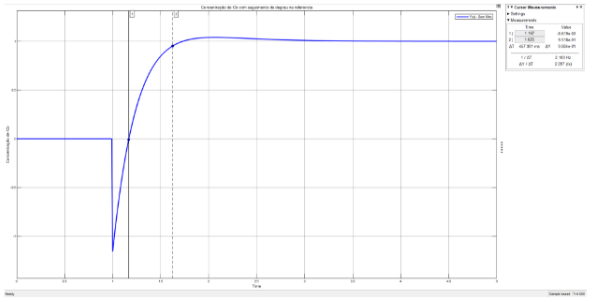
\includegraphics[width=0.8\linewidth]{Imagens/Grafico com mf na entrada.png}
    \caption{Resposta de MF com degrau na entrada (Sem filtro)}
    \label{fig:enter-label}
\end{figure}

Desenvolvendo o Diagrama de Pólos e Zeros da resposta em relação à referência sem o filtro:

\begin{figure}[H]
    \centering
    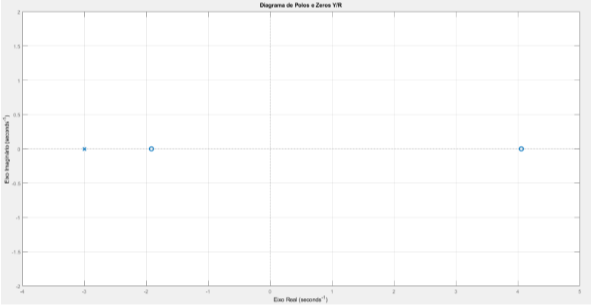
\includegraphics[width=0.8\linewidth]{Imagens/polo e zero sem filtro.png}
    \caption{Resposta de MF com degrau na entrada (Sem filtro)}
    \label{fig:enter-label}
\end{figure}

Analisando o diagrama de pólos e zeros da em relação à referência sem o filtro, percebe-se a presença de um zero dominante que causa um sobresinal, e também um zero presente no semiplano direito que causa uma fase não-mínima na resposta. Ambas características podem ser vistas na figura 18 da resposta em relação a referência. 

Agora, plota-se o gráfico da resposta para a referência com a introdução do filtro:

\begin{figure}[H]
    \centering
    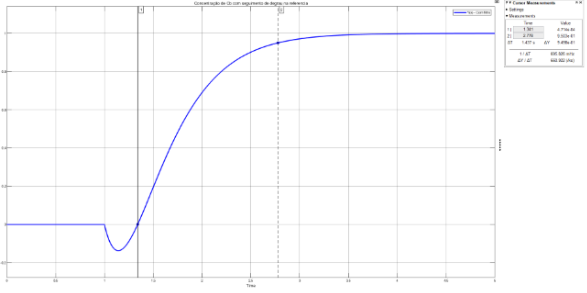
\includegraphics[width=0.8\linewidth]{Imagens/resposta.png}
    \caption{Resposta de MF com degrau na entrada (Com filtro)}
    \label{fig:enter-label}
\end{figure}

Para entender de onde surge as características da resposta, analisa-se o diagrama de pólos e zeros, que é visto abaixo:

\begin{figure}[H]
    \centering
    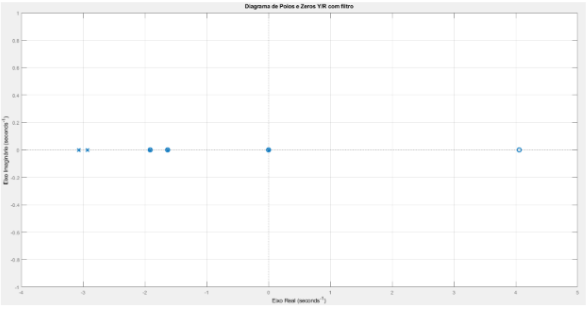
\includegraphics[width=0.8\linewidth]{Imagens/polo e zero com filtro.png}
    \caption{Diagrama de pólos e zeros Y/R com filtro}
    \label{fig:enter-label}
\end{figure}


Como pode-se observar, o efeito do zero dominante é inibido pela presença do polo do filtro, fazendo com que não haja mais o sobressinal na resposta. Porém, é visto que a presença do zero no semiplano direito continua, sendo assim, ainda há a presença da fase não-mínima que pode ser observada na figura 20 . 

Partimos agora, para a análise da resposta à perturbação, da qual obtemos o seguinte gráfico:

\begin{figure}[H]
    \centering
    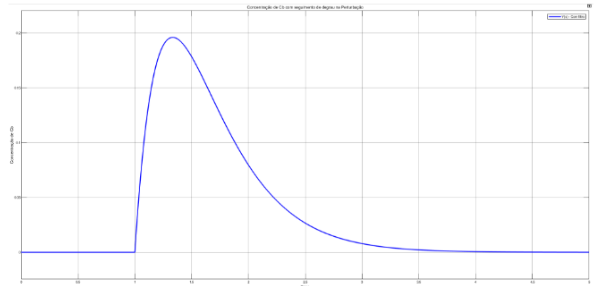
\includegraphics[width=0.8\linewidth]{Imagens/resposta mf com degrau.png}
    \caption{Resposta de MF com degrau de perturbação}
    \label{fig:enter-label}
\end{figure}

Para auxiliar o entendimento de onde surge as características da resposta, analisa-se o diagrama de pólos e zeros, que é visto abaixo:

\begin{figure}[H]
    \centering
    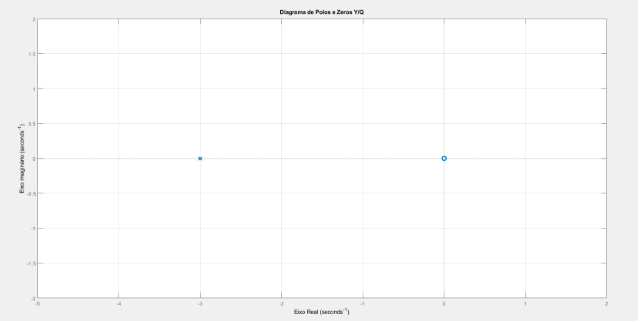
\includegraphics[width=0.5\linewidth]{diagramapolosezeros.png}
    \caption{Diagrama de polos e zeros Y/Q }
    \label{fig:enter-label}
\end{figure}

Analisando o diagrama de pólos e zeros da resposta em relação a perturbação, percebe-se que o sobressinal da resposta surge do zero dominante.  


No geral, primeiramente é visto que a introdução do filtro na malha fechada foi essencial, pois de fato realizou a retirada do sobressinal aparente nas respostas do sistema em relação a referência. Além do mais, observa-se que a dinâmica do sistema simulado apresentou um ganho unitário, perceptível quando o sistema tende a zero logo após a introdução de uma perturbação. Além do mais, a presença do zero causador da fase não mínima acabou por gerar uma resposta mais lenta, ou seja, o tempo de assentamento foi maior do que o desejado. Porém, ao ser descontado o tempo dessa fase não-mínima é possível observar que o valor do tempo de assentamento se apresenta muito próximo da faixa de valor desejado. Para este zero causador de fase não-mínima não foi possível fazer com que seu efeito seja cancelado pelo controlador e nem pelo filtro de referência.   

Entretanto, existe a possibilidade de se obter respostas mais rápidas para o sistema, porém, para realizar tal mudança é necessário alterar as raízes do polinômio desejado e assim obter um novo polinômio de malha fechada, o que alteraria a resposta do sistema. Contudo, para realizar tais mudanças é necessário realizar uma verificação dos limites do sistema físico, uma vez que essas mudanças poderiam causar respostas muito agressivas para os dispositivos que operam no sistema real.  

Vamos agora analisar o diagrama de bode da resposta em relação a referência:

\begin{figure}[H]
    \centering
    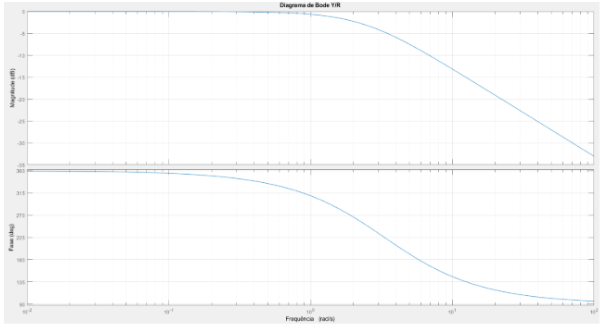
\includegraphics[width=0.8\linewidth]{Imagens/bodey.png}
    \caption{Diagrama de bode de Y/R}
    \label{fig:enter-label}
\end{figure}

través do diagrama de bode da resposta em relação a referência acima é percebido um comportamento muito interessante, o qual passa a reduzir sinais com frequências maiores do que 1 rad / s. Dessa forma, assemelhando-se muito à um filtro passa-baixa, que é capaz de permitir sinais de frequências menores e diminuir efeitos de sinais que apresentam maiores frequências. 

Analisa-se agora o diagrama de bode da resposta em relação a perturbação:

\begin{figure}[H]
    \centering
    \includegraphics[width=0.8\linewidth]{Imagens/pertubaçao.png}
    \caption{Diagrama de bode de Y/Q}
    \label{fig:enter-label}
\end{figure}

A partir do diagrama de bode acima, da resposta frente a perturbação, é visto que sinais com frequências pertencentes a uma certa faixa de valor tem maior magnitude, fora dessa faixa de frequência os valores desses sinais são minimizados. Portanto, o comportamento dessa resposta se assemelha muito a um filtro Passa-Faixa, que tem a capacidade de rejeitar sinais fora de uma faixa de frequência especificada, enquanto permite a passagem dos sinais com frequência dentro dessa faixa.



\section{8) Simulação do Comportamento Dinâmico em Simulink}

Usando Simulink, estude por simulação o comportamento dinâmico do sistema em frequência com o modelo completo não linear e verifique se atende as especificações. Implemente um cenário de simulação com a partida do sistema em rampa até chegar no ponto de operação. Simule, então, variações perto do ponto de operação e aplique perturbações. Poderia obter respostas mais rápidas? Por quê? O que acontece com o sistema ao se afastar do ponto de operação?

Implementando o sistema de controle no simulink no sistema não linear, obtivemos o seguinte diagrama de blocos.

\begin{figure}[H]
    \centering
    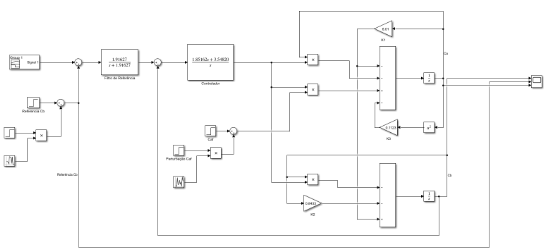
\includegraphics[width=0.8\linewidth]{diagramablocos.png}
    \caption{Diagrama de blocos do sistema não linear com o controlador e filtro}
    \label{fig:enter-label}
\end{figure}

Neste diagrama, o gerador de sinais utiliza uma rampa para levar o sistema ao ponto de operação, e então o sinal tipo rampa é desligado. O tempo necessário para levar o sistema ao ponto de operação foi de 8 segundos, após este tempo, o sinal de referência é ligado e então o sistema de controle passa a atuar mantendo o sistema no ponto de operação. 

\begin{figure}[H]
    \centering
    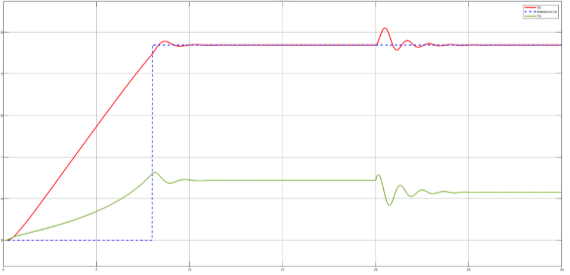
\includegraphics[width=0.8\linewidth]{naolinear.png}
    \caption{Resposta do sistema não linear com controlador e filtro e perturbação em Caf}
    \label{fig:enter-label}
\end{figure}

Na figura acima é possível verificar o funcionamento do sistema de controle, onde este é capaz de levar a concentração de Cb ao valor desejado, mesmo após inserirmos a perturbação em Caf no tempo t = 20 min. 

\begin{figure}[H]
    \centering
    \includegraphics[width=0.8\linewidth]{respostacompequenasvariaçoes.png}
    \caption{Resposta do sistema não linear com controlador e filtro com pequenas variações de referência e perturbações em Caf}
    \label{fig:enter-label}
\end{figure}

No gráfico acima é possível ver o sistema rejeitando perturbações e pequenas mudanças de referência, o que é o comportamento esperado para o sistema de controle projetado.
 Elevando um pouco a variância do sinal de referência Cb, começamos a ver que o sistema tem um pouco de dificuldade de responder corretamente, mas ainda consegue seguir o valor da referência.
 
\begin{figure}[H]
    \centering
    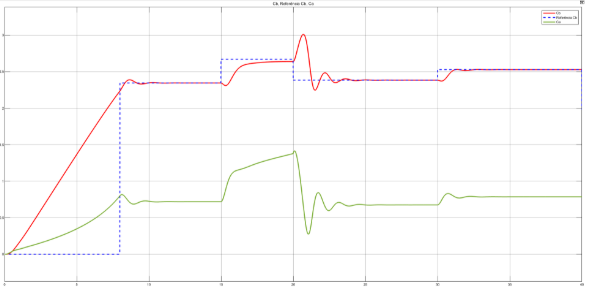
\includegraphics[width=0.8\linewidth]{respostacomcontrolador.png}
    \caption{Resposta do sistema não linear com controlador e filtro com variações médias na referência e perturbações em Caf}
    \label{fig:enter-label}
\end{figure}

Elevando ainda mais a variância do sinal de referência, podemos verificar que a não linearidade do processo começa a afetar o sistema, com a concentração de Cb não convergindo para o valor de referência. Portanto o sistema deve atuar somente com pequenas variações na referência. 

\begin{figure}[H]
    \centering
    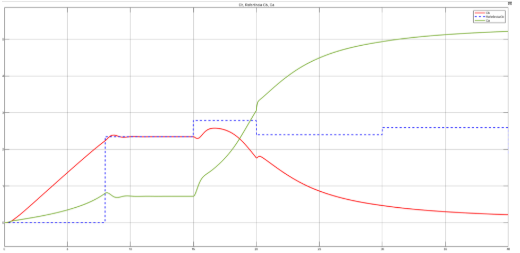
\includegraphics[width=0.8\linewidth]{respostaaosistemanaolinear.png}
    \caption{Resposta do sistema não linear com controlador e filtro com variações grandes na referência.}
    \label{fig:enter-label}
\end{figure}

Com respeito a velocidade do processo, seria possível obter respostas mais rápidas ao reduzir o tempo de assentamento, ou seja, calculando os pólos desejados novamente, utilizando a planta linearizada e selecionando outros parâmetros do controlador. Porém, fica a ressalva de que antes de implementar essas modificações referentes a aceleração das respostas, é necessário compreender os limites físicos do processo e então encontrar o tempo mínimo de assentamento que não resulte num sinal de controle muito agressivo, capaz de danificar os maquinários utilizados no processo real.

 Outro ponto a ser levado em consideração é a não linearidade do processo, pois podemos encontrar dificuldades em acelerar a resposta do sistema de controle e manter a coerência do modelo não linear e do modelo linearizado, já que para acelerar o processo o sistema de controle teria de aumentar a magnitude do sinal de controle, podendo levar o sistema não linear para uma faixa de operação diferente da qual o sistema foi linearizado, impossibilitando a estabilidade do sistema, semelhante ao ocorrido na figura 2.26.


\section{9) Controle Discreto}

Discretize o controle do ponto 1, escolhendo adequadamente \( T_s \). Implemente o controle em MATLAB, escrevendo o código de controle. Simule um cenário onde o sistema é levado até o ponto de operação em modo MANUAL e somente então o controle passa a AUTOMÁTICO. Usando ferramentas no domínio da frequência, analise o seu controle discretizado e compare com o contínuo. Analise o efeito da amostragem.

Sabendo que o tempo de amostragem a ser utilizado é:

\[
Ts =\frac{1.6}{20} = 0.08
\]

Utilizando o método Forward, onde: 

\[
s =\frac{(z-1)}{Ts}
\[

Temos que a discretização do nosso controlador se dará da seguinte forma:

\[
C(s) =\frac{1.85162s+3.54820}{s} = \frac{1.85162\frac{z-1}{Ts}+3.54820}{\frac{z-1}{Ts}}
\]

\[
\frac{\frac{1.85162}{Ts}(z-1)+3.54820}{\frac{z-1}{Ts}} . \frac{Ts}{Ts}=\frac{1.85162 z - 1 + 3.54820Ts}{z-1}

\]

\[
C(z)=\frac{1.85162z - 1.85162 + 3.54820Ts}{z-1}
\]

Também é necessário realizar a discretização do filtro:

\[
Fr(s)=\frac{1.91627}{(s + 1.91627)}=\frac{1.91627}{\frac{z-1}{Ts}+ 1.91627}.\frac{Ts}{Ts}
\]


\[
Fr(z) = \frac{1.91627Ts}{z - 1 + 1.91627Ts}
\]

Pelo diagrama de blocos temos que:

\[
C=\frac{U}{E}= \frac{1.85162z - 1.85162 + 3.54820Ts}{z-1}
\]

Dessa forma, temos que a equação de diferenças é:

\[

U(k) - U(k - 1) = 1.85162E(k) - 1.85162E(k - 1) + 3.54820TsE(k - 1)

U(k) = 1.85162E(k) + (- 1.85162 + 3.54820Ts)E(k - 1) + U(k - 1)

\]

E para o filtro temos:

\[
Fr=\frac{Rf}{R} = \frac{1.91627Ts}{z - 1 + 1.91627Ts}

\]

Rf(k) - Rf(k - 1) + 1.91627Ts Rf(k - 1) = 1.91627Ts R(k - 1)

Rf(k) = 1.91627Ts R(k - 1) + (1 - 1.91627Ts)Rf(k - 1)

\[



Utilizando \( C_a \) e \( C_b \) como:

\]

C_a(k + 1) = (-k_1C_a(k) - u(k)C_a(k) - k_3C_a\power{2}k + C_{a_f}(k)u( k) )Tc + C_a(k)

C_b(k+1) = (k_1C_a(k) - k_2C_b(k) - C_b(k)u(k))Tc + C_b(k)


\[


Criamos o seguinte código no matlab:

\begin{lstlisting}[language=Matlab, caption={Exemplo de codigo MATLAB}, label={lst:matlab}]
close all
clear
clc
Ts = 0.08;
% -------------------- Sinal de Referencia ------------------------
t_final = 50; % tempo total de simulacao
t = 0:Ts:t_final; % vetor de tempo
t_rampa = 8; % duracao da rampa
rampa_slope = 2.5 / t_rampa; % inclinacao da rampa
rampa_offset = 0; % valor inicial da rampa
rampa_final_value = 2.345; % valor final apos a rampa
R = rampa_slope .* (t - rampa_offset) .* (t <= t_rampa) +
rampa_final_value .* (t > t_rampa);
R(t >= 25) = 2.15; % mudanca de valor a partir de T = 20
plot(t, R, 'LineWidth', 2, 'Color', 'red');
hold on;
% --------------------- Perturbacao Caf ---------------------------

caf = 5.1*ones(size(t)); % vetor inicialmente com valor 5.1 para todos
os tempos
caf(t >= 40) = 4.5; % mudanca de valor a partir do tempo t = 25
%inicializacao das variaveis do processo
k1=6.01;
k2=0.8433;
k3=0.1123;
nit = round(t_final/Ts); % numero de iteracoes do laco de controle

Ca = zeros(1,nit+1);
Cb = zeros(1,nit+1);
U = zeros(1,nit+1);
rfant = 0;
eant = 0; % como o sistema e ligado desde o inicio, todos sao zero
uant = 0;

%Laco de Controle
for k=2:nit+1
% sistema de controle
y = Cb(k-1);
%rf = 0.1533016*R(k-1) + 0.8466984*rfant;
rf = 1.91627*Ts*R(k-1)+ (1-1.91627*Ts)*rfant;
e = rf - y;
%u = 1.85162*e - 1.567764*eant + uant;
u = 1.85162*e + (-1.85162+3.54820*Ts)*eant + uant;
% saturacao do sinal de controle
if u >= 10
u = 10;
end
if u <= 0
u = 0;
end
U(k-1) = u; % para o plot do sinal de controle
% atualizacao das variaveis de controle
uant = u;
eant = e;
rfant = rf;
% simulacao do processo com modelo nao linear

Ca(k)=(-k1*Ca(k-1)-u*Ca(k-1)-k3*((Ca(k-1))^2)+caf(k-
1)*u)*Ts+Ca(k-1);

Cb(k)= (k1*Ca(k-1)-k2*Cb(k-1)-Cb(k-1)*u)*Ts+Cb(k-1);

end
% plot sinais de referencia, ca e cb
plot(t, Cb, 'LineWidth', 2, 'Color', 'blue');
plot(t, Ca, 'LineWidth', 2, 'Color', 'green');
grid on;
legend('Referencia', 'Cb', 'Ca');
xlabel('Tempo [min]');
ylabel('Concentracao [mol/l]');
title('Concentracao de Cb e Ca com Referencia Para Cb e Perturbacao em
Caf');

% plot principais sinais
figure();
plot(t, U, 'LineWidth', 2, 'Color', 'blue');
hold on
plot(t, caf, 'LineWidth', 2, 'Color', 'red');
plot(t, Cb, 'LineWidth', 2, 'Color', 'black');
plot(t, R, 'LineWidth', 2, 'Color', 'green', 'LineStyle', '--');
legend('Sinal de Controle u', 'Perturbacao de Caf', 'Concentracao de
Cb', 'Referencia');
grid on;
title('Principais Sinais');
xlabel('Tempo [min]');
ylabel('Amplitude');
\end{lstlisting}


Obtivemos os seguintes gráficos com a execução do código e Ts=0.08, em 40 min, ocorre uma perturbação de Caf para vermos como o sistema lida com isso:

\begin{figure}[H]
    \centering
    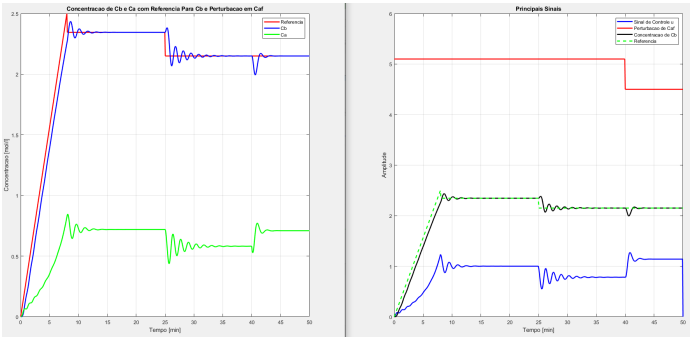
\includegraphics[width=0.8\linewidth]{figurats.png}
    \caption{Ts = 0.08}
    \label{fig:enter-label}
\end{figure}

Se alterarmos o valor de Ts para 0.04, percebemos que o sistema leva menos tempo para atingir a região permanente:

\begin{figure}[H]
    \centering
    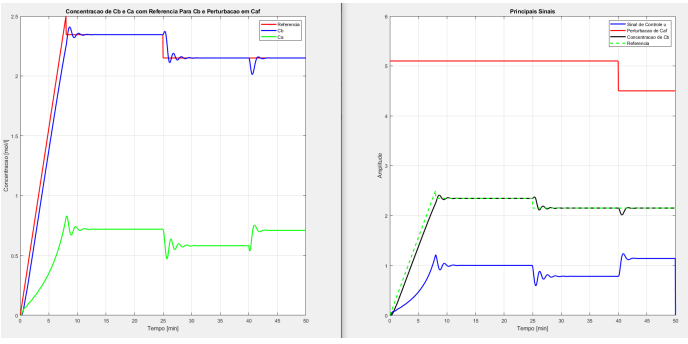
\includegraphics[width=0.8\linewidth]{FiguraTsnovo.png}
    \caption{Ts = 0.04}
    \label{fig:enter-label}
\end{figure}

Se alterarmos o valor de Ts para 0.1, percebemos que o sistema leva mais tempo para atingir a região permanente:

\begin{figure}[H]
    \centering
    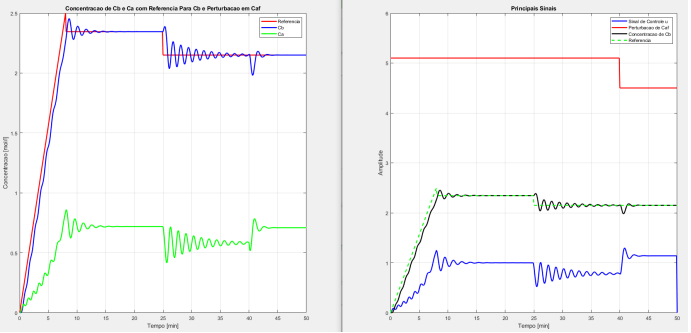
\includegraphics[width=0.8\linewidth]{Ts01.png}
    \caption{Ts = 0.1}
    \label{fig:enter-label}
\end{figure}


Podemos perceber que o sistema com o controle discretizado é um pouco mais instável
do que o sistema contínuo, isso se dá devido ao uso da aproximação Forward, que é uma
aproximação com uma maior taxa de erro.
  
  \end{document}